% Graduation Thesis Template for HCMUS students
% Adapted for English-language thesis: "uMatter: A Microservices-Based
% Mental Health Support Platform for Teenagers"
% Based on the official KLTN template (bhthong@fit.hcmus.edu.vn)

% NOTE (build order): delete all files generated by a previous build, then
% build in this order: BIB > PDF > PDF. Rebuild the same way whenever the
% bibliography changes.

\documentclass[oneside,a4paper,14pt]{extreport}

% Fonts
% NOTE: the original HCMUS template uses [T5]{fontenc} for Vietnamese
% diacritics. Since this thesis body is written in English, T1 is used
% instead; switch back to T5 (and install the vntex/texlive-lang-other
% packages) if you reintroduce Vietnamese text (e.g., a Vietnamese abstract).
\usepackage[T5]{fontenc}
\DeclareTextSymbolDefault{\DH}{T1}
\usepackage[utf8]{inputenc}

\usepackage{tabularx}

% Bibliography
\usepackage[style=ieee]{biblatex}
\usepackage[unicode]{hyperref} % Vietnamese-safe bookmarks
\addbibresource{References/references.bib}

\makeatletter
\def\blx@maxline{77}
\makeatother

% Images (kept in Images/)
\usepackage{graphicx}
\graphicspath{ {Images/} }

% Source code listings
\usepackage{listings}
\usepackage{color}
\definecolor{codegreen}{rgb}{0,0.6,0}
\definecolor{codegray}{rgb}{0.5,0.5,0.5}
\definecolor{codepurple}{rgb}{0.58,0,0.82}
\definecolor{backcolour}{rgb}{0.95,0.95,0.92}
\lstdefinestyle{mystyle}{
    backgroundcolor=\color{backcolour},
    commentstyle=\color{codegreen},
    keywordstyle=\color{magenta},
    numberstyle=\tiny\color{codegray},
    stringstyle=\color{codepurple},
    basicstyle=\footnotesize,
    breakatwhitespace=false,
    breaklines=true,
    captionpos=b,
    keepspaces=true,
    numbers=left,
    numbersep=5pt,
    showspaces=false,
    showstringspaces=false,
    showtabs=false,
    tabsize=2
}
\lstset{style=mystyle}

% Pseudocode
\usepackage{amsmath}
\usepackage{algorithm}
\usepackage[noend]{algpseudocode}
\makeatletter
\def\BState{\State\hskip-\ALG@thistlm}
\makeatother

% Tables
\usepackage{multirow}
\usepackage{array}
\newcolumntype{L}[1]{>{\raggedright\let\newline\\\arraybackslash\hspace{0pt}}m{#1}}
\newcolumntype{C}[1]{>{\centering\let\newline\\\arraybackslash\hspace{0pt}}m{#1}}
\newcolumntype{R}[1]{>{\raggedleft\let\newline\\\arraybackslash\hspace{0pt}}m{#1}}

% English default names (change back to Vietnamese if your program requires it)
\renewcommand{\chaptername}{Chapter}
\renewcommand{\figurename}{Figure}
\renewcommand{\tablename}{Table}
\renewcommand{\contentsname}{Table of Contents}
\renewcommand{\listfigurename}{List of Figures}
\renewcommand{\listtablename}{List of Tables}
\renewcommand{\appendixname}{Appendix}

% Chapter heading size
\usepackage{titlesec}
\titleformat{\chapter}[display]
  {\LARGE\bfseries}
  {\chaptertitlename\ \thechapter}{18pt}{\huge}

% 1.5 line spacing
\usepackage{setspace}
\onehalfspacing

% First-line indent
\usepackage{indentfirst}

% Margins
\usepackage[
  top=30mm,
  bottom=25mm,
  left=30mm,
  right=20mm,
  includefoot]{geometry}

% Cover page
\usepackage{tikz}
\usetikzlibrary{calc}
\newcommand\HRule{\rule{\textwidth}{1pt}}

% ========================================================================================= %
% NOTE: general thesis information - fill these in before your final build                  %
% ========================================================================================= %
\newcommand{\tenSV}{Dương Trung Hiếu - Dương Ngọc Quang Khiêm} % non-breaking space between name parts
\newcommand{\mssv}{22125027~-~22125037}
\newcommand{\tenKL}{uMatter:An Application for Supporting Mental Health}
\newcommand{\tenGVHD}{PGS.TS Nguyễn Văn Vũ}
\newcommand{\tenBM}{BACHELOR OF SCIENCE IN COMPUTER SCIENCE}

\begin{document}

\begin{titlepage}
\begin{center}

{\large VIETNAM NATIONAL UNIVERSITY, HO CHI MINH CITY}\\
{\large UNIVERSITY OF SCIENCE}\\
{\large FACULTY OF INFORMATION TECHNOLOGY}\\[0.3cm]

\HRule \\[0.4cm]

% Replace with the official faculty/university logo, e.g.:
% \includegraphics[width=3cm]{logo_hcmus.png}

\vspace{1.5cm}

\tenSV \\
\mssv \\[1.2cm]

{\Huge \bfseries \tenKL \par}

\vspace{1.2cm}

{\large GRADUATION THESIS}\\
{\large \tenBM}

\vspace{1.5cm}

{\large Advisor: \tenGVHD}

\vfill

{\large Ho Chi Minh City, \the\year}

\end{center}
\end{titlepage}

% After the title page, insert the (signed) advisor's and reviewer's
% comments, which are provided by the Faculty's academic affairs office
% after the defense, so the final bound copy can include them.

\cleardoublepage

\pagenumbering{roman} % i, ii, iii, ...

\phantomsection
\chapter*{Statement of Originality}
\label{commitment}

I hereby declare that this is my own research, carried out under the supervision of \tenGVHD. The data and results presented in this thesis are truthful and have not been duplicated from any other work.


% \addcontentsline{toc}{chapter}{Statement on Topic Revisions}
% \chapter*{Statement on Topic Revisions}
\label{edit}

Statement describing any revisions made after the defense (e.g., changes to the thesis title or report content), if applicable.


% \addcontentsline{toc}{chapter}{Advisor's Comments}
% \chapter*{Advisor's Comments}
\label{advisor}

The advisor's signed comment sheet, provided by the academic affairs office.


% \addcontentsline{toc}{chapter}{Reviewer's Comments}
% \chapter*{Reviewer's Comments}
\label{reviewer}

The reviewer's signed comment sheet, provided by the academic affairs office.


\addcontentsline{toc}{chapter}{Acknowledgments}
\chapter*{Acknowledgments}
\label{thanks}

We would first like to express our sincere gratitude to our advisor,
\tenGVHD, for his guidance, patience, and constructive criticism throughout
every stage of this thesis. We are equally grateful to our reviewer for taking
the time to read this work carefully and for the comments that improved it.
% TODO: after the reviewer (GVPB) is assigned, replace the phrase above with
% their full name and title, e.g. "to our reviewer, TS. <Name>,".

This thesis would not have taken the shape it did without the mental-health
professionals who agreed to advise a student project. We thank
\textbf{Ms. Phạm Thị Thanh Quí}, counsellor at the Psychological Counselling
Office, University of Science, VNU-HCM; \textbf{Mr. Vương Nguyễn Toàn Thiện},
CEO of LUMOS, the psychology organization accompanying the Faculty of
Information Technology in 2026; and \textbf{Dr. Phạm Trần Thành Nghiệp},
physician at Hoàn Mỹ Sài Gòn Hospital, a partner of the Faculty of Information
Technology from 2022 to 2025.

We are also grateful to the friends who took part in the first round of
user-story interviews, and who returned months later for the closed testing and feedback
round to tell us honestly what did and did not work. Their time was given
freely and their criticism was given generously.

Finally, we thank the Faculty of Information Technology and the University of
Science, VNU-HCM, for the resources, the coursework, and the feedback that made
this project possible, and our families, for their patience and support
throughout the development of uMatter.


% \addcontentsline{toc}{chapter}{Thesis Proposal}
% \chapter*{Thesis Proposal}
\label{proposal}

The approved thesis proposal, previously submitted to the academic affairs office \textit{(must bear the advisor's signature)}.


% TOC, list of figures, list of tables
\addcontentsline{toc}{chapter}{Table of Contents}
\tableofcontents

% \cleardoublepage
% \addcontentsline{toc}{chapter}{\listfigurename}
% \listoffigures

\cleardoublepage
\addcontentsline{toc}{chapter}{\listtablename}
\listoftables

\addcontentsline{toc}{chapter}{Abstract}
\chapter*{Abstract}
\label{summary}

Adolescent mental health support remains fragmented: self-care tools including mood or sleep trackers such as Daylio, Wysa and Bearable, rarely connect to licensed professional care, while therapy platforms such as BetterHelp and Talkspace typically specialize in only finding you a trusted therapist without giving the therapist enough context as to how you are doing in order to efficiently conduct meaningful sessions. And while there are platforms for people to have deep conversations with close friends and family, it is hard for parents to actually know how their children are doing and feeling. And as a trend of young people seeking mental health advice from AI, a centralized platform where the user can choose to share their daily reflective tracking data with AI would be more beneficial in case they truly want a deeply contextual advice instead of a vague one. This gap motivates a platform that unifies these fragmented features so that the user don't have to spend unnecessary time explaining themselves every time they want to use  a feature from a different platform, providing the best mental health support as we can.

This thesis presents uMatter, a mental health support platform for teenagers that combines self-care features, an AI companion, peer social features as well as professional therapy features.

uMatter is implemented as a microservices system: seven Spring Boot services (authentication, tracking, AI, dashboard, therapist, social, and notification) sit behind an Nginx API gateway, communicate asynchronously through RabbitMQ, and follow a database-per-service pattern backed by PostgreSQL, Redis, and MinIO. Access control uses stateless JWT authentication with a JWKS-published RSA key and a permission-based data-sharing model so users can selectively grant professionals access to their tracked data. The AI companion is grounded in each user's own tracking history and served through Google's Gemini 2.5 Flash. The system was hardened through structured security audits covering injection risks, insecure direct object references, and mass assignment, and a database-level atomic slot claim, backed by a unique constraint, was introduced to close a race condition in appointment booking. The full stack was deployed and validated on cloud infrastructure, running as 20 containers.

The resulting platform demonstrates that a unified self-care and professional therapy experience can be successfully delivered through a single, security-conscious microservices architecture. However, as an academic prototype, uMatter scopes out key real-world operational challenges. It excludes legal and compliance frameworks, dispute resolution mechanisms for handling user or therapist conflicts, and the monetization model essential for incentivizing licensed professionals. Despite these out-of-scope administrative limitations, this thesis establishes a robust technical foundation. Future work can build upon this architecture by integrating monetization systems, comprehensive legal safeguards, clinical collaboration requirements, and layered risk detection, ultimately advancing uMatter toward a fully viable ecosystem for adolescent mental health support.

\clearpage

\pagenumbering{arabic} % 1, 2, 3, ...

% Content chapters
\chapter{Introduction}
\label{Chapter1}

\section{Background and Motivation}

Adolescent mental health in Vietnam has become a problem that needs more attention than ever. In recent years a ninth-grader in Ho Chi Minh City took his own
life after a poor exam result~\cite{DanTri2017}, and a final-year Information
Technology student at the University of Science, VNU-HCM died the same way~\cite{TuoiTre2024}. These are not isolated: a cross-sectional
study of 1{,}316 high-school students across six districts of Ho Chi Minh City
found that 46.5\% reported self-injury behaviour~\cite{PhamThao2019}, and the
global picture agrees the World Health Organization estimates that one in
seven adolescents aged 10-19 experiences a mental disorder, accounting for 15\%
of the disease burden in this age group, with suicide the third leading cause of
death among those aged 15-29~\cite{WHO_AdolescentMH}. What makes such cases so
difficult to accept is that the distress is rarely invisible in hindsight. It is
usually present beforehand, in ordinary conversations and small changes of
behaviour, and simply never seen by anyone positioned to act. The signal exists;
nothing is holding it.

Yet the tools available to a teenager today address only fragments of this
problem. On one side of the market, self-care applications such as Daylio and
Bearable let users log their mood, sleep, and daily activities, helping them
notice patterns in their own well-being~\cite{Daylio, Bearable}. These tools are
lightweight and approachable, but they stop at self-observation: they do not
connect a user who needs help to a licensed professional. On the other side,
therapy-oriented platforms such as BetterHelp and Talkspace connect users with
licensed therapists for text, audio, or video counseling~\cite{BetterHelp,
Talkspace}, while AI-first platforms such as Wysa offer a conversational
companion alongside optional access to coaches~\cite{Wysa}. These platforms are
targeted primarily around adults, and around one side of the care
journey, either self-tracking or professional therapy.
The consequence is that a therapist meets a patient with no context beyond what
that patient can reconstruct from memory in the room, and a parent has no way of
knowing how their child is actually doing.

\subsection*{What we learned from users}

To find where these tools fail in practice, we ran a baseline study in which a
psychology student at HCMUE, a Business student at
RMIT, evaluated ten existing platforms: AI chatbots,
trackers, peer communities, telehealth services, and clinical software
against two personas: an undergraduate diagnosed with mild-to-moderate
depression, and a tenth-grader under academic pressure whose family does not
believe anything is wrong. Four findings shaped this thesis. First, the week
between sessions is a black box: by the appointment, what the patient
meant to discuss is forgotten or too exhausting to reconstruct. Second,
input fatigue was the single most cited reason for abandoning a health
app. Third, tracking alone produced no progress;
trackers were judged useful for noticing patterns and worthless for changing
them, while an AI companion was seen as genuinely supportive but never a
substitute for a human professional. Fourth, privacy is a precondition,
not a feature: the strongest reaction concerned data leaking at the moment the
user is most vulnerable, and willingness to share was never absolute a
journal could go to a therapist but not to friends, and an automatic crisis
alert to family was rejected outright as pressure to perform a better mood than
the one being felt.

\subsection*{What we learned from professionals}

We then consulted three mental-health professionals: a counsellor from the
Psychological Counselling Office at the University of Science, VNU-HCM; the CEO
of the psychology organization LUMOS; and a physician at Hoàn Mỹ Sài Gòn
Hospital. Their guidance shaped the product directly: replacing periodic
surveys with a continuous emotion timeline captured every few hours, because
daily reflection yields richer and more meaningful data than any questionnaire;
routing a user who logs anger toward a breathing exercise and a user who logs
sadness toward their stored positive memories; and treating physical activity,
sleep, and nutrition as inseparable from mental well-being.

 Two of the three were
substantially opposed to AI in mental health: one holding that an AI should
answer only the easiest questions and should never be given access to a user's
personal tracking data at all, while the third supported it, carefully
applied, as a genuine source of companionship. One was openly distrustful of
peer connection, on the grounds that a well-meaning friend may offer advice that
runs directly against clinical guidance, and recommended that such connections
be limited to parents and preceded by explicit warnings. As a result, every audience including the AI companion, a
therapist, a trusted friend or parent, must be granted access explicitly, in
scope, and revocably, with nothing shared by default.

\subsection*{Why we built this}

Finally, and most plainly: the two of us wanted to help. We are not clinicians,
and this thesis does not pretend to treat anyone. But we can build software, and
much of what is missing is a software problem somewhere for a young person's
daily reality to be captured comfortably enough that it actually gets captured,
and a controlled path from that record to the people who can help, whether that
is an AI at 3 AM, a friend, a parent, or a licensed therapist.


\section{Problem Statement}
\label{sec:problems}


\subsection*{Problem 1: Eliciting the data}

\textit{How can a platform obtain an honest, continuous record of a teenager's mood,
emotions, and daily wellbeing in a way that feels natural and comfortable rather than
like clinical paperwork?}

The ideal solution would be \textit{implicit}: inferring emotional state from signals the
user already produces, without asking them to report anything. The motivating case is: before a recent suicide by a secondary-school student in Ho Chi Minh City \cite{DanTri2017}, the
warning was present in ordinary conversations with friends; had it been noticed, it might
have been acted upon. But capturing that class of signal means continuously listening to
real-life conversations, reading messaging apps, or monitoring facial expressions around
the clock. Such surveillance is technically fragile, ethically indefensible for minors,
and in direct conflict with data-protection law.
That decision converts Problem 1 into a design problem: self-report is only useful if it
actually happens, day after day, and self-report is exactly what users abandon first.
The difficulty is threefold:

\begin{itemize}
\item \textbf{Friction.} Every second of effort between "I feel something" and "it is
recorded" costs data. Capture must be a single tap, expanded only if the user wants to
elaborate.
\item \textbf{Recall and initiation.} A teenager in a low mood is the least likely person
to remember to open a wellbeing app. The system must come to the user rather than wait
for them, without becoming a nag that gets muted or uninstalled.
\end{itemize}

This thesis addresses Problem 1 through a set of \textbf{daily reflection and tracking}
features designed as one habit rather than ten tools: a one-tap \textbf{mood check-in}
(\textit{Cảm xúc lúc này}) across five levels with an optional line of context; an
\textbf{emotional journal} (\textit{Góc tâm tư}) for free-form reflection with photos, a
mood calendar, and streaks; and \textbf{wellbeing logs} for sleep, nutrition and water,
and breathing with step count collected automatically, the one passive signal that
requires no surveillance of the user's private life. Elicitation itself is handled by
\textbf{Focus Mode}, which nudges roughly every 90 minutes during waking hours and
respects a Quiet Hours window, so the record accumulates without the user having to
remember to build it.

\subsection*{Problem 2: Acting on the data}

\textit{Given that record, how can the platform tell whether a user is in distress, act appropriately when they are, and still be worth opening when they are not? Resolving this requires nuanced interpretation to distinguish acute distress from an ordinary bad day or a long-term downward trend. Furthermore, because most days are simply neutral or mildly negative, a platform built only for crises will remain closed on an average day. Finally, navigating these states safely demands strict data sensitivity, ensuring that any access to a user's mood, sleep, and journal data is always explicit and revocable, rather than granted by default.}

In crisis, a dedicated emergency-support area always one tap away. For the ordinary day, the same record powers an AI companion whose
replies are grounded in how the user has actually been sleeping and feeling, guided
breathing and meditation, a Treasure Box of pre-saved positive memories to
reopen when recall of the good is hardest, and lightweight achievements that make the
habit itself rewarding.

The two problems close a loop: better daily reflection makes every downstream response
more precise, and responses that are genuinely useful on ordinary days are what keep the
reflection going.

\section{Objectives}
\label{sec:objectives}


\subsection*{Capturing the record (Problem 1)}

\begin{itemize}
  \item O1 Make capture experience as comfortable as possible.

  \item O2 Bring the system to the user without becoming a nag.

  \item O4 Cover physical wellbeing as the consulted professionals framed
    it
\end{itemize}

\subsection*{Acting on the record (Problem 2)}

\begin{itemize}
  \item O5 Ground the AI companion in the user's own history

  \item O6 Respond appropriately to the ordinary day, through
    guided breathing and meditation, a Treasure Box of pre-saved positive
    memories surfaced when recall of the good is hardest, emotion-appropriate
    routing (anger toward breathing, sadness toward stored memories), and
    lightweight achievements and streaks that make the habit itself rewarding.

  \item O7 Keep the crisis path one tap away

  \item O8 Close the black box between sessions
\end{itemize}

\subsection*{Consent, architecture, and validation}

\begin{itemize}
  \item O9 Share nothing by default.

  \item O10 Build the system as a maintainable microservices
    architecture

  \item O11 Demonstrate that the result runs, by deploying and
    validating the full stack on cloud infrastructure.
\end{itemize}

\section{Scope}
\label{sec:scope}


uMatter is built as an academic prototype: a working system, deployed and
exercised end to end, whose purpose is to demonstrate that the unified
experience can be delivered
through a single coherent architecture. Its intended users are Vietnamese
adolescents, with the audiences they may choose to admit, an AI companion, a licensed therapist, a parent, or a friend. Within that, the thesis covers the daily reflection and tracking features,
the responses built on top of them, the permission model governing who may see
what, the seven-service backend and its supporting infrastructure, and the
deployment of the whole stack to cloud infrastructure.

Several concerns that a production deployment would have to address are
deliberately excluded, and are treated in 
future work rather than as gaps in the implementation:

\begin{itemize}
  \item \textbf{Legal and regulatory compliance.} Data-protection obligations,
    consent law for minors, and the licensure requirements governing
    teletherapy are outside the scope of this thesis. 

  \item \textbf{Dispute resolution.} The platform provides no mechanism for
    adjudicating conflicts between a user and a therapist, or between users.

  \item \textbf{Monetization.} No payment, billing, or compensation model is
    implemented. This is not a missing feature: without it there is no
    incentive structure to attract licensed professionals to the platform.

  \item \textbf{Clinical validation.} uMatter makes no diagnostic claim and was
    not evaluated in a clinical trial. No assertion is made that the platform
    improves mental-health outcomes; the evaluation concerns the system, not its
    therapeutic efficacy.

  \item \textbf{Automated risk detection.} The platform does not attempt to
    infer crisis from the tracked record and does not escalate on the user's
    behalf. The emergency-support path is user-initiated by design, a
    decision reinforced by our baseline study, in which an automatic crisis
    alert to family was rejected outright as pressure to perform a better mood
    than the one being felt. 


\end{itemize}

\section{Contributions}

This thesis makes the following contributions:

\begin{itemize}
  \item \textbf{A unified platform.} uMatter integrates daily reflective
    tracking, an AI companion, peer and family connection, and professional
    therapy into a single system, so that a user need not re-explain themselves
    each time they cross from one fragment of the existing market into another.

  \item \textbf{A consent model.} The permission-based data-sharing design, in which every
    audience is granted access explicitly, in scope, and revocably, with nothing
    shared by default.


  \item \textbf{Requirements grounded in primary study.} The design is
    driven by a baseline evaluation of ten platforms against two
    personas, conducted with a psychology student at HCMUE, and by consultation
    with three mental-health professionals. The findings are reported and traced to the features they produced.

    \item \textbf{A pioneering localized prototype.} As one of the first native 
    applications tailored specifically for adolescent mental health in Vietnam, uMatter raises 
    critical awareness about the well-being of Vietnamese teenagers and young adults. It provides 
    a meaningful, usable prototype demonstrating that mental health can be supported in many connected ways, with the help of yourself and the people around who truly care about you, embodying the platform's core message: \textit{you matter}.

\end{itemize}

 % Introduction
\chapter{Related Work}
\label{Chapter2}

The Abstract and Chapter~\ref{Chapter1} describe adolescent mental-health support today as fragmented across four kinds of tools. This chapter surveys each of these four fragments in turn, positions uMatter relative to them, and reviews the architectural and security literature that informs the design presented in Chapter~\ref{Chapter3}.

\section{Self-Care and Tracking Applications}

Daylio and Bearable are representative of a category of lightweight, single-purpose self-care applications~\cite{Daylio,Bearable}. Daylio focuses on quick, low-friction mood and activity logging, encouraging habit formation through streaks and reminders. Bearable extends this idea to a broader set of symptoms and factors (sleep, medication, exercise, weather, and more), letting users explore correlations in their own data.

Both applications are valuable for self-observation, but neither connects a user to a professional: there is no booking, matching, or clinical workflow, and the data collected has no path out of the app other than manual export. For a teenager who identifies a concerning pattern in their own tracked data, these tools offer no next step, and our own baseline study found the same limitation from the user's side: trackers were judged useful for noticing patterns and worthless for changing them.

\section{Professional Therapy Platforms}

BetterHelp and Talkspace sit at the opposite end of the spectrum~\cite{BetterHelp,Talkspace}. Both connect users with licensed therapists through a subscription model, primarily via asynchronous messaging with optional live sessions. Their onboarding is built around a short intake questionnaire used to match a new user to a therapist, and their core workflows (scheduling, secure messaging, video sessions) are mature and well-tested at scale.

These platforms are built for a general adult audience, and they do not provide day-to-day self-care tracking as a first-class feature - a user's mood or sleep history is not something the platform helps them build up over time outside of a therapy session. A therapist on these platforms meets a patient with no context beyond what that patient can reconstruct from memory in the room, which is precisely the black-box week our baseline study identified as a recurring failure. These platforms also do not target the specific constraints of a teenage user base, such as guardian involvement or age-appropriate content and matching.

\section{Social and Family Connection Platforms}

A third fragment is not a mental-health product at all, but the general-purpose messaging and social platforms a teenager already uses to talk to friends and family. In Vietnam, this is overwhelmingly Zalo, the country's leading messaging platform~\cite{Zalo}, alongside global platforms such as Messenger. These platforms are conversational infrastructure, not wellbeing infrastructure: they carry whatever a teenager chooses to say, but they do not structure that conversation around mood or wellbeing, and they give a parent no visibility into how their child is actually doing beyond what that child volunteers to share.

Family-oriented applications such as Life360 address a related but different problem, surfacing a family member's location and presence rather than their emotional state~\cite{Life360}, so a parent can confirm that their child arrived home safely without learning anything about how the child felt that day. This is precisely the gap our professional consultations surfaced: a parent has no way of knowing how their child is actually doing. It is also why our own consulted professionals disagreed on how far peer and family connection should go at all, one warning that a well-meaning friend's advice can run against clinical guidance, which is why uMatter treats a parent or friend as an audience that must be explicitly and revocably granted access, rather than a channel that is open by default.

\section{General-Purpose AI for Mental Health Advice}

A fourth fragment is not a product category but a documented behavior: adolescents and young adults increasingly turn to general-purpose AI chatbots, ChatGPT, Google Gemini, Meta AI, and similar tools, when they feel sad, angry, or nervous. A nationally representative U.S. survey found that roughly one in eight adolescents and young adults aged 12 to 21 had used a generative-AI chatbot for mental health advice, with the large majority of those users rating the advice helpful~\cite{2025-McBain-GenAI}. Wysa is the most mature purpose-built instance of this same pattern, wrapping a conversational AI companion around a mental-health-specific design, with an optional paid tier that adds access to human coaches~\cite{Wysa}.

What both the general-purpose chatbots and Wysa share, from uMatter's perspective, is that neither is grounded in a continuous, structured record of the user's own life: a general-purpose chatbot starts from nothing every conversation, and Wysa's companion, while mental-health-aware, does not draw on a user's own logged mood, sleep, or journal history at all. uMatter's own companion can draw on that history, but only once the user has explicitly granted it access through the same permission model used for a therapist (Section~\ref{sec:datasec}); absent that grant, it converses without grounding rather than reading tracking data by default. The same survey work that documents this trend also cautions that there are few standardized benchmarks for the quality of the mental-health advice these systems provide, which echoes what our own consulted professionals insisted on: an AI companion should never substitute for a human professional, and, for at least one of the three we consulted, should not be given access to a user's personal tracking data at all.

\section{Positioning of uMatter}

Table~\ref{tab:competitive} summarizes this comparison across all four fragments surveyed above: self-care tracking, professional therapy, social and family connection, and AI-based advice-seeking. uMatter's distinguishing position is that it treats these as four aspects of one continuous user journey rather than four separate products a teenager must adopt and re-explain themselves, connected by a permission-based data-sharing model in which a user's own tracked history travels only where they explicitly allow it: to a matched therapist, to a parent or friend, or to the AI companion itself, with nothing shared by default.

\begin{table}[ht]
\caption{Feature comparison between uMatter and comparable platforms}
\label{tab:competitive}
\begin{center}
\renewcommand{\arraystretch}{1.5}
\setlength{\tabcolsep}{6pt}
\begin{tabular}{ |L{3.4cm}|C{2.6cm}|C{2.6cm}|C{2.6cm}|C{2.6cm}| }
 \hline
 \textbf{Feature} & \textbf{uMatter} & \textbf{BetterHelp / Talkspace} & \textbf{Wysa / General AI Chatbots} & \textbf{Daylio / Bearable} \\
 \hline
 Mood/sleep/journal tracking & Yes & No & Partial & Yes \\
 \hline
 AI companion grounded in own data & Yes & No & No (general) & No \\
 \hline
 Licensed therapist matching \& booking & Yes & Yes & Limited & No \\
 \hline
 Video consultation & Yes & Yes & No & No \\
 \hline
 Clinical notes for professionals & Yes & Yes & No & No \\
 \hline
 Peer social features & Yes & No & No & No \\
 \hline
 Parent/guardian visibility (with consent) & Yes & No & No & No \\
 \hline
 Teen-oriented design & Yes & No & Partial & Partial \\
 \hline
 Granular, permission-based data sharing & Yes & N/A & N/A & N/A \\
 \hline
\end{tabular}
\end{center}
\end{table}

\section{Architectural Foundations}

The system architecture proposed in Chapter~\ref{Chapter3} builds on well-established distributed-systems practice rather than novel architectural research. The decomposition into independently deployable services, each owning its own data store, follows the microservices style described by Newman~\cite{2021-Newman-Microservices}, chosen over a monolithic design because uMatter's functional areas (authentication, tracking, AI, professional workflows, social features, notifications) have different scaling, security, and change-rate profiles. Inter-service communication uses a mix of synchronous REST calls, following the architectural constraints of the REST style~\cite{2000-Fielding-REST}, and asynchronous messaging through RabbitMQ for event-driven workflows~\cite{RabbitMQ}. Services are implemented with Spring Boot~\cite{SpringBoot} and packaged with Docker~\cite{Docker} to keep the development and deployment environments consistent.

\section{Security Foundations}

Securing a distributed system requires standards-based authentication and proactive threat modeling. Modern architectures favor stateless, token-based authentication via JSON Web Tokens (JWT)~\cite{2015-RFC7519-JWT}, verified cryptographically through JSON Web Key Sets (JWKS)~\cite{2015-RFC7517-JWK} to eliminate centralized session bottlenecks. System design is typically benchmarked against consensus frameworks like the OWASP Top 10~\cite{2021-OWASP-Top10} to proactively mitigate critical vulnerabilities such as Broken Access Control and Injection flaws.

Beyond authentication, robust authorization relies on formal access control models. While Role-Based Access Control (RBAC)~\cite{1996-Sandhu-RBAC} efficiently manages coarse-grained permissions, Attribute-Based Access Control (ABAC) ~\cite{2014-NIST-ABAC} is necessary for fine-grained, ownership-driven data sharing. To enforce these models safely, security literature emphasizes the principle of Defense in Depth~\cite{1975-Saltzer-Schroeder}. Access rules are embedded declaratively at the method level.

\section{AI Companion And Video Consultation}

The in-app AI companion is powered by the Gemini API from Google, utilizing the Gemini 2.5 Flash model~\cite{2024-Gemini-TechReport}. Unlike a general-purpose chatbot, the companion is grounded in the user's own tracking history, so its responses can refer to a user's recently logged mood, sleep, or journal entries rather than operating from a blank context. Video consultation between users and therapists is facilitated through Jitsi Meet~\cite{Jitsi} public meeting rooms on the internet, providing an open-source video-conferencing solution that avoids dependence on a proprietary video vendor. % Related Work
\chapter{System Analysis and Design}
\label{Chapter3}

\section{Requirements Analysis}
\label{sec:requirements}

uMatter has four direct actors: the primary user, can be the teenager who
is seeking support for mental health or a close friend and family,
who tracks their wellbeing on the mobile application and owns every piece of
data they produce; the
therapist, working from the web dashboard; and the
administrator. Importantly, a teen may admit to their tracked record:
therapists, parents and close friends (other user accounts), the AI companion, all subject to the same explicit, scoped, revocable grants
(Section~\ref{sec: data}).

\begin{table}[htbp]
  \centering
  \caption{Key functional requirements and the objectives they realize}
  \label{tab:freq}
  \begin{tabular}{|l|p{8.2cm}|l|}
    \hline
    \textbf{ID} & \textbf{Requirement} & \textbf{Obj.} \\
    \hline
    FR1 & One-tap five-level mood check-in with optional context; journal
          with photos, mood calendar, and streaks. & O1, O6 \\
    \hline
    FR2 & Logs for sleep, nutrition and water, and breathing; step count is
          collected automatically and is the only passive signal. & O3, O4 \\
    \hline
    FR3 & Focus Mode prompts a check-in roughly every 90 minutes during
          waking hours, silent during user-configured Quiet Hours. & O2 \\
    \hline
    FR4 & The AI companion grounds its replies in the user's own tracking
          data if and only if the user has granted it access. & O5, O9 \\
    \hline
    FR5 & Guided breathing and meditation, and a Treasure Box of saved
          positive memories, routed to by logged emotion; an emergency
          area reachable in one tap from anywhere. & O6, O7 \\
    \hline
    FR6 & Therapist discovery, appointment booking, video consultation, and
          clinical notes; tracked data visible to a therapist only under an
          explicit, scoped, revocable grant. & O8, O9 \\
    \hline
    FR7 & Friend and parent connections with real-time chat; a connection by
          itself exposes no tracked data. & O9 \\
    \hline
    FR8 & Domain events produce push, email, and in-app notifications to the
          affected parties. & O2, O8 \\
    \hline
  \end{tabular}
\end{table}

\begin{table}[htbp]
  \centering
  \caption{Key non-functional requirements}
  \label{tab:nfreq}
  \begin{tabular}{|l|p{8.2cm}|l|}
    \hline
    \textbf{ID} & \textbf{Requirement} & \textbf{Obj.} \\
    \hline
    NFR1 & Privacy by default. No tracked data is visible to any
           audience without an active grant, enforced server-side so a
           compromised client cannot bypass it. & O9 \\
    \hline
    NFR2 & Stateless security. RSA-signed JWTs validated locally by
           every service against a published JWKS key. & O10 \\
    \hline
    NFR3 & Integrity under concurrency. Concurrent bookings of the
           same slot must not both succeed; retried requests are not applied
           twice. & O8 \\
    \hline
    NFR4 & Independent evolvability on modest infrastructure. Each
           service develops, deploys, and migrates independently, and the
           full platform runs on a single cloud virtual machine. & O10, O11 \\
    \hline
  \end{tabular}
\end{table}


\section{Overall Architecture}

\begin{figure}[htbp]
    \centering
    % Assuming your main.tex is at the root directory, you need the full path
    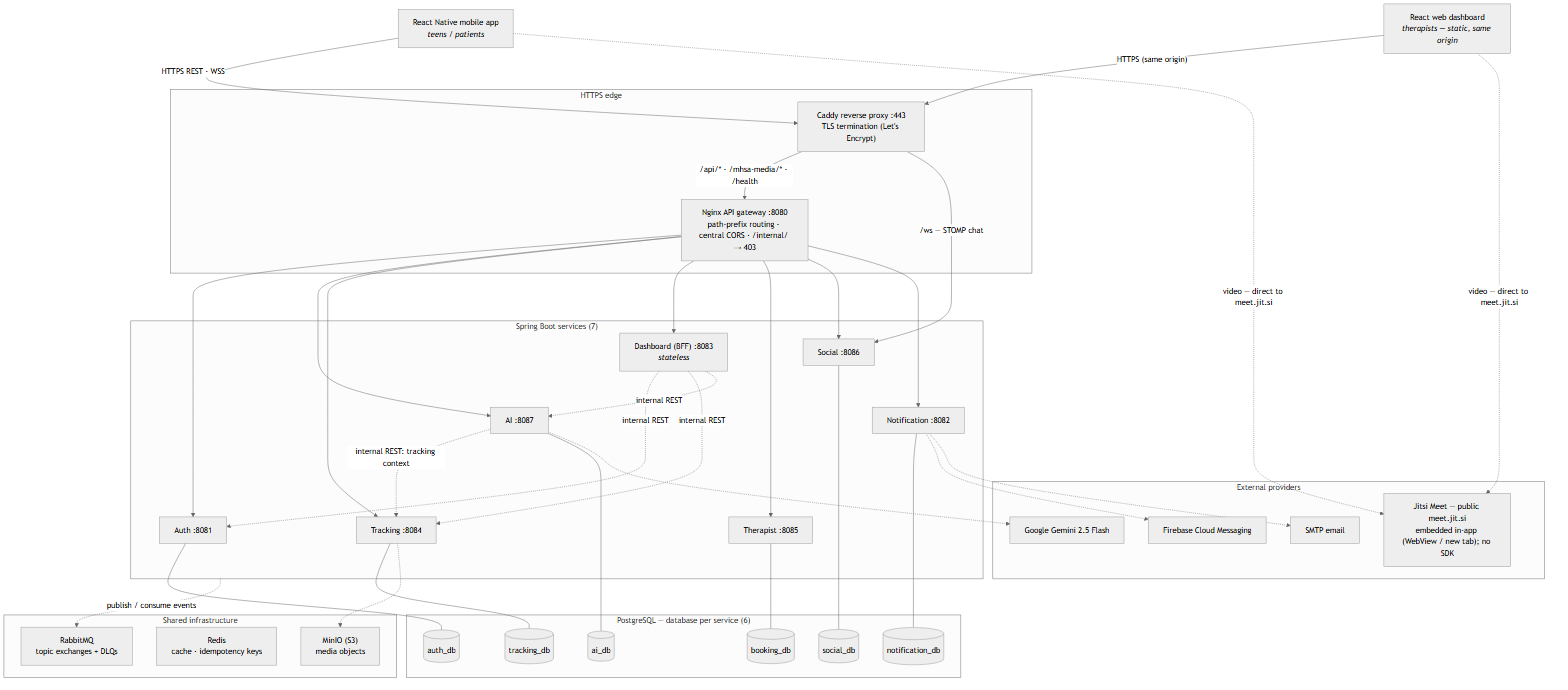
\includegraphics[width=\textwidth]{Chapter3/images/ch3-overall-architecture.png}
    \caption{The overall microservices architecture of uMatter.}
    \label{fig:ch3_overall_architecture}
\end{figure}

uMatter follows a microservices architecture: independently deployable Spring Boot services sit behind a single Nginx API gateway, which is the only entry point reachable by the two client applications - a React Native mobile app for teenagers/patients and a React web dashboard for therapists. The gateway is responsible for routing requests to the correct backend service and for terminating HTTPS at the edge of the system.

This decomposition is not free, and for a two-person academic project the
choice deserves justification. We accept the operational overhead of seven
deployables, a message broker, and per-service databases in exchange for
two things. First, independent lifecycles, which are not hypothetical here:
the services live in separate repositories, evolving without
coordinated upgrades. Second, each service is scoped to a single functional area, can be developed, deployed, and scaled independently, and owns its own data.

This decomposition follows the pattern described by Newman~\cite{2021-Newman-Microservices}, synchronous request/response interactions between services and clients use REST-style HTTP APIs~\cite{2000-Fielding-REST}; workflows that are naturally asynchronous, such as sending a notification after an event happens elsewhere in the system, are handled through RabbitMQ instead~\cite{RabbitMQ}.

\section{Service Decomposition}

The backend is organized into seven services, summarized in Table~\ref{tab:services}.

\begin{table}[ht]
\caption{uMatter backend services and their responsibilities}
\label{tab:services}
\begin{center}
\begin{tabular}{ |L{2.6cm}|L{9.5cm}| }
 \hline
 \textbf{Service} & \textbf{Responsibility} \\
 \hline
 Auth & User registration/login, JWT issuance and refresh, JWKS key publication, role management \\
 \hline
 Tracking & Mood, sleep, and journal entry storage; the source of truth for a user's self-reported well-being data \\
 \hline
 AI & Manages conversations with the AI companion, grounding responses in the user's own tracking data \\
 \hline
 Dashboard & Aggregates tracking data into summaries and visual trends for the user \\
 \hline
 Therapist & Therapist discovery/matching, appointment booking, video consultation session management, clinical notes \\
 \hline
 Social & Peer relationships (friends) and real-time chat over STOMP/WebSocket \\
 \hline
 Notification & Consumes domain events and delivers push (FCM), email, and in-app inbox notifications \\
 \hline
\end{tabular}
\end{center}
\end{table}


\section{Data Architecture}
\label{sec: data}

uMatter follows a database-per-service pattern: each backend service owns a private PostgreSQL database, and no service reaches directly into another service's schema. Cross-service data needs are satisfied either through a synchronous API call to the owning service or through an asynchronous event, never through shared tables. This keeps each service free to evolve its own schema without coordinating a migration across the whole system, at the cost of needing an explicit strategy (API calls or events) for any data that spans services.

Two supporting stores complement PostgreSQL:

\begin{itemize}
\item \textbf{Redis} is used for caching and for idempotency keys, so that a retried request (for example, a client retry after a network timeout) is not applied twice.
\item \textbf{MinIO}, an S3-compatible object store, holds binary media such as profile photos and any files attached to journal entries or clinical notes, keeping large binary payloads out of the relational databases.
\end{itemize}

To prevent synchronous bottlenecks when one service frequently requires data owned by another, the system utilizes an event-driven replication strategy via RabbitMQ topic exchanges. As illustrated in Figure~\ref{fig:ch3-replication-events}, the architecture maintains four primary replication streams: the Therapist API replicates auth-owned therapist profiles; the Tracking Service maintains a local replica of data access grants (serving as the consent gate for patient data); the Auth service replicates patient-therapist assignments; and the Social service listens for active assignments to automatically provision direct chat channels between patients and their therapists.

To ensure data integrity and fault tolerance across these asynchronous boundaries, all replication consumers implement a strict set of resilience patterns. Consumers utilize manual acknowledgments and operate as a single consumer per queue to maintain reliable processing. Message failures are routed to a Dead Letter Exchange and Queue (DLX/DLQ) for debugging and replay. Furthermore, to safely handle duplicate message deliveries, consumers enforce database-watermark idempotency based on an \texttt{occurredAt} timestamp. Finally, to guarantee eventual consistency and recover from any prolonged messaging outages, a nightly reconciliation process synchronizes the replica tables against an internal snapshot provided by the data owner.

\begin{figure}[htbp]
    \centering
    
    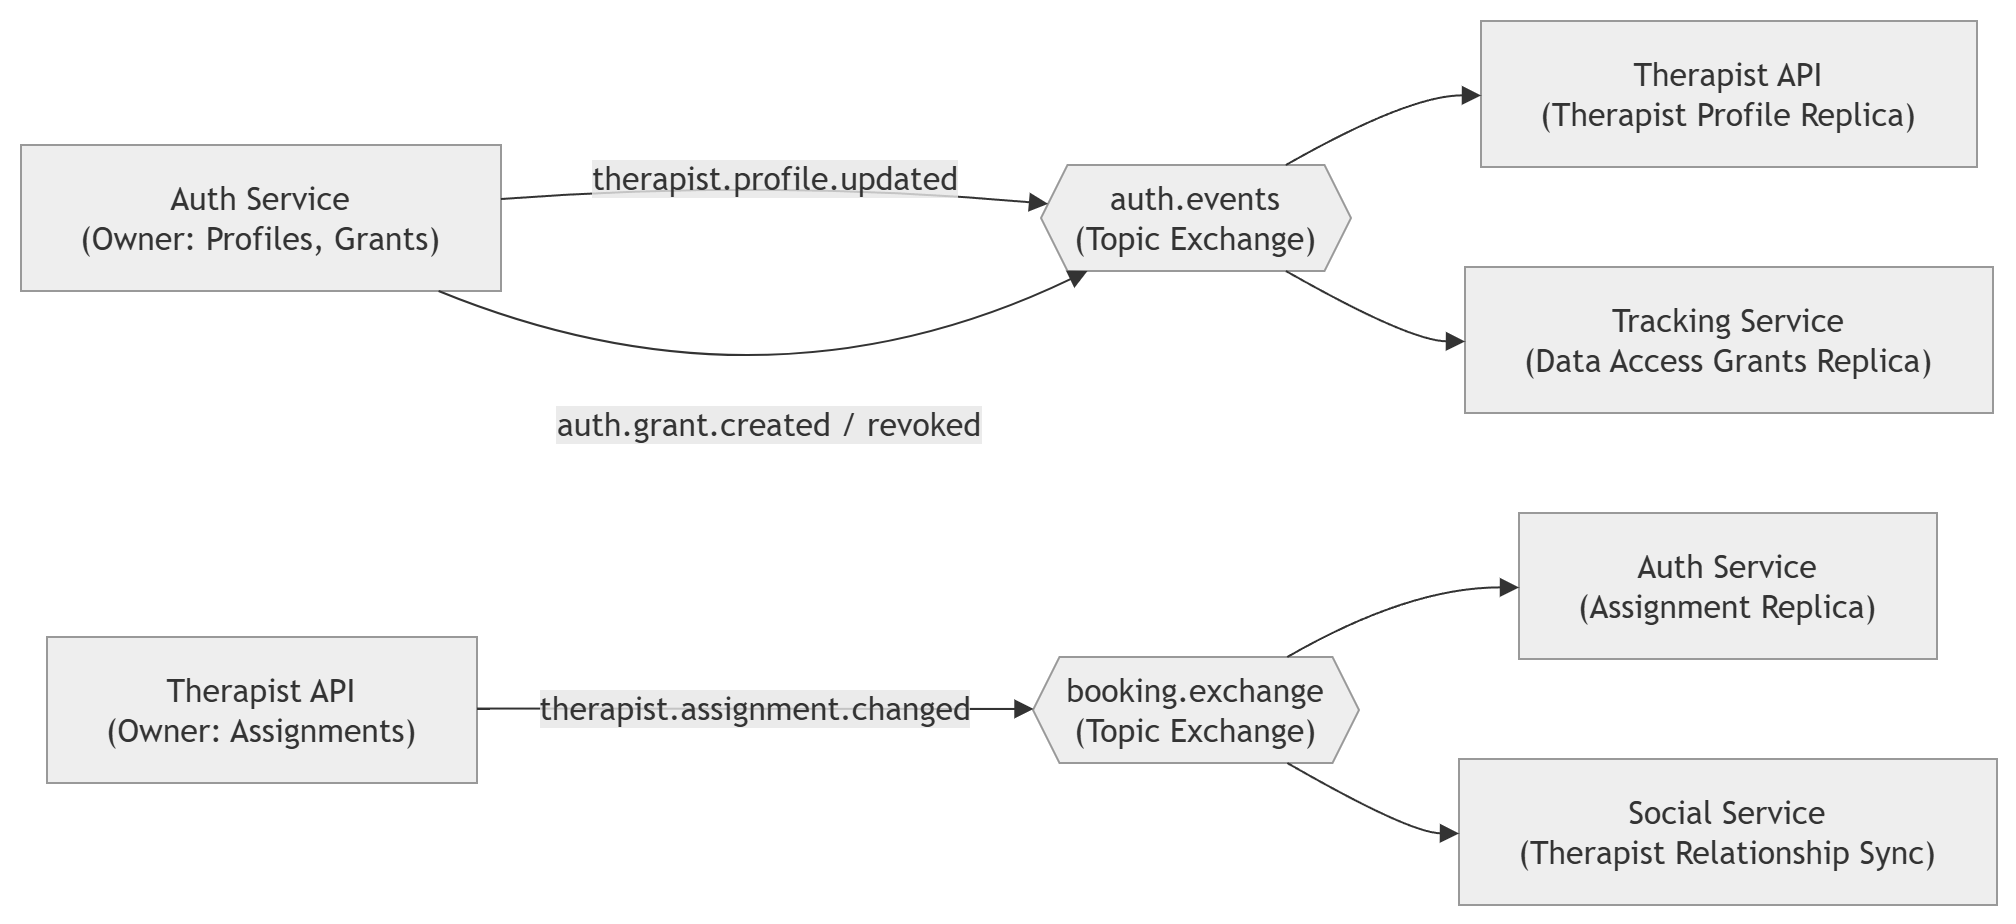
\includegraphics[width=0.8\textwidth]{Chapter3/images/ch3-replication-events.png}
    \caption{The four replication streams}
    \label{fig:ch3-replication-events}
\end{figure}

\section{Authentication, Authorization, and Data Sharing}
\label{sec:datasec}

\begin{figure}[htbp]
    \centering
    
    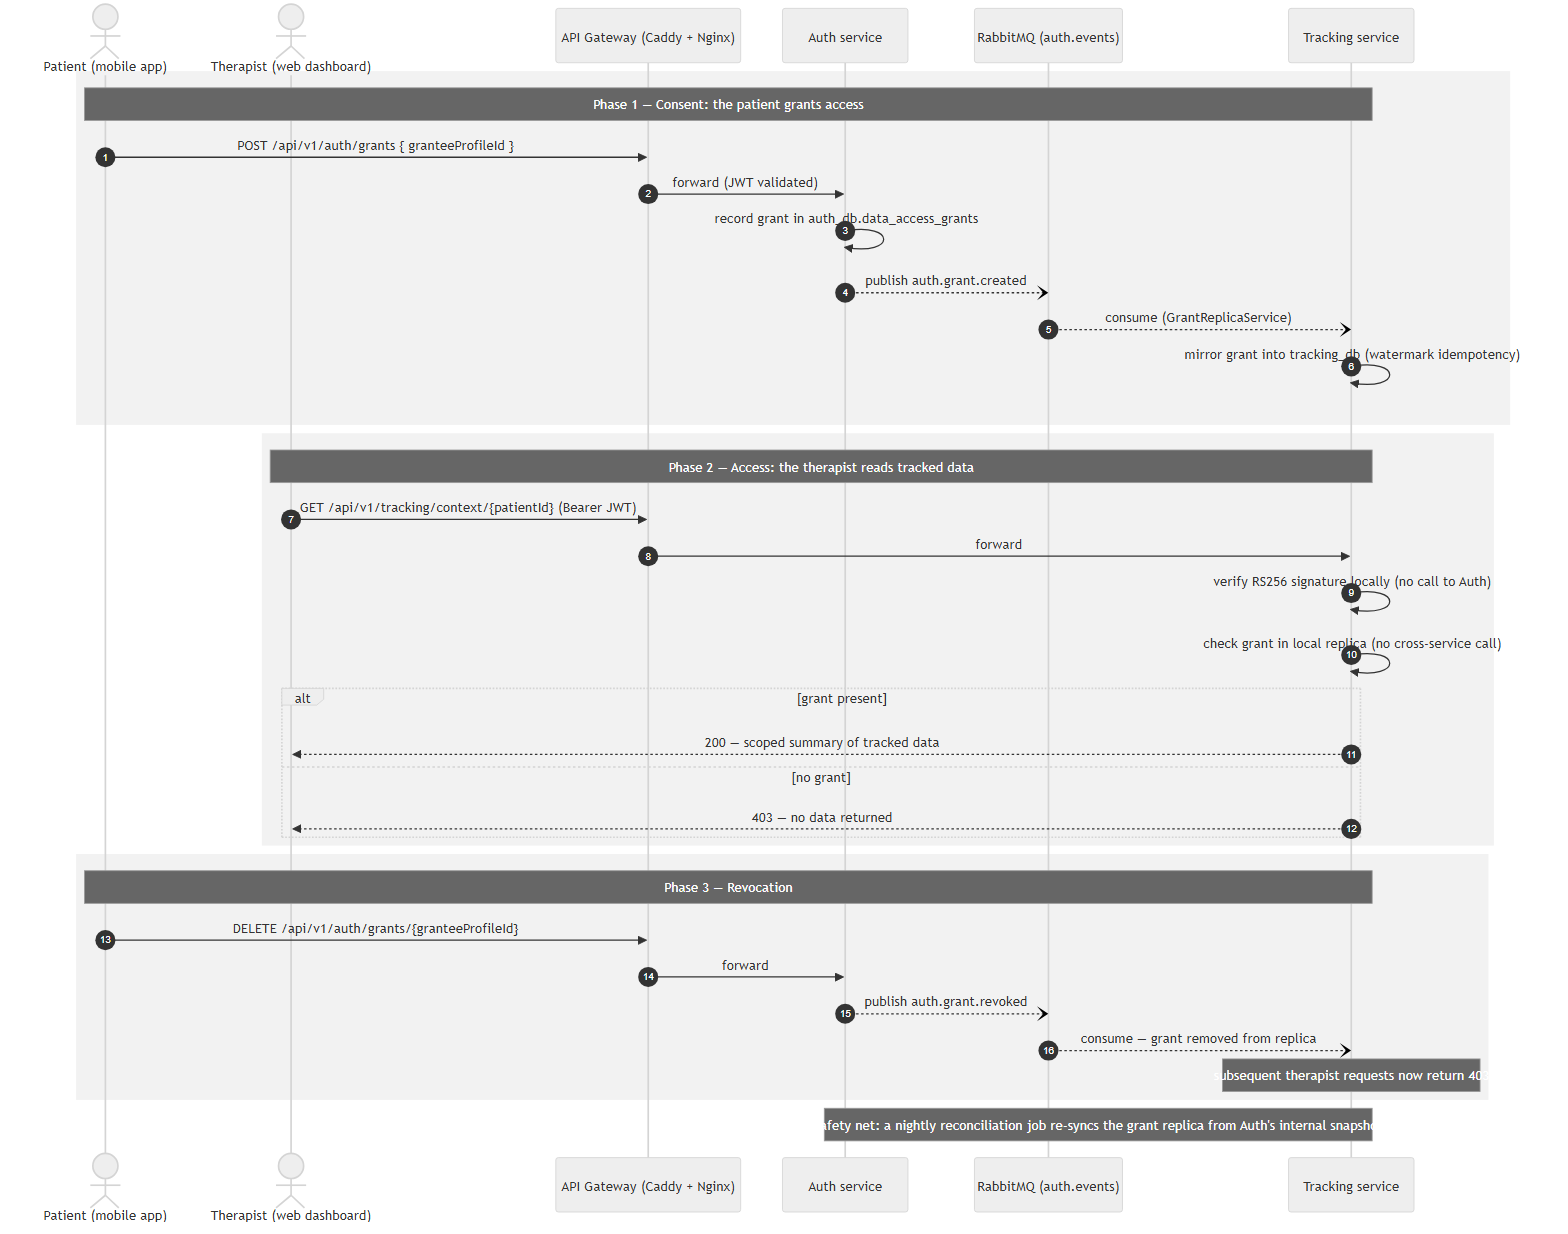
\includegraphics[width=\textwidth]{Chapter3/images/ch3-permission-grant-flow.png}
    \caption{A sequence diagram of a permission-checked data access.}
    \label{fig:ch3-permission-grant-flow}
\end{figure}

Authentication is stateless: the Auth service issues JSON Web Tokens signed with an RSA private key, following RFC 7519~\cite{2015-RFC7519-JWT}, and publishes the corresponding public key through a JWKS endpoint. Every other service validates incoming tokens locally against this published key, so no service needs to call back to Auth (or share a session store) simply to authenticate a request. Roles embedded in the token (teen/patient, therapist, admin) drive coarse-grained authorization at the gateway and service level.

Fine-grained authorization is handled by a permission-based data sharing model, which is central to uMatter's design goal of not exposing sensitive tracked data by default. A user's mood, sleep, food, journal, step, and breathing records are private to that user unless the user explicitly grants another party access. A grant names a \emph{set of tracking categories} it covers, so a user may share, for example, their sleep and nutrition but withhold their journal, carries a thirty-day expiry, and is revocable at any time. Enforcement lives at the Tracking service boundary: every read of a category is gated on an active, unexpired grant whose scope set includes that category, checked against a locally replicated copy of the grants (Section~\ref{sec:events}) rather than left to the client application, so that a compromised or misbehaving client cannot bypass it. The same mechanism serves every audience uniformly: a therapist, a parent, a friend, and the AI companion are all grantees enforced by identical code.

Service-to-service calls follow a two-tier trust model. User-facing APIs
(\texttt{/api/**}) always require a valid JWT, validated locally by the
receiving service. Internal APIs (\texttt{/internal/**}) --- such as the
Tracking endpoint the AI service calls to assemble conversation context, or
the grant snapshot the Tracking service pulls from Auth during nightly
reconciliation --- do not carry the user's token; the caller passes the
subject's profile identifier explicitly. These endpoints are protected by
network topology instead: they are reachable only on the private container
network, and the gateway refuses any external request whose path begins with
\texttt{/internal/}. Asynchronous messaging is likewise authenticated at the
broker with per-deployment RabbitMQ credentials. The trade-off is that any
process on the internal network is trusted; mutual TLS or per-service
credentials would remove that assumption and are noted as future hardening,
but within a single-host deployment where the internal network is not shared
with third-party workloads, perimeter trust is a proportionate design.

\section{AI Companion}

\begin{figure}[htbp]
    \centering
    
    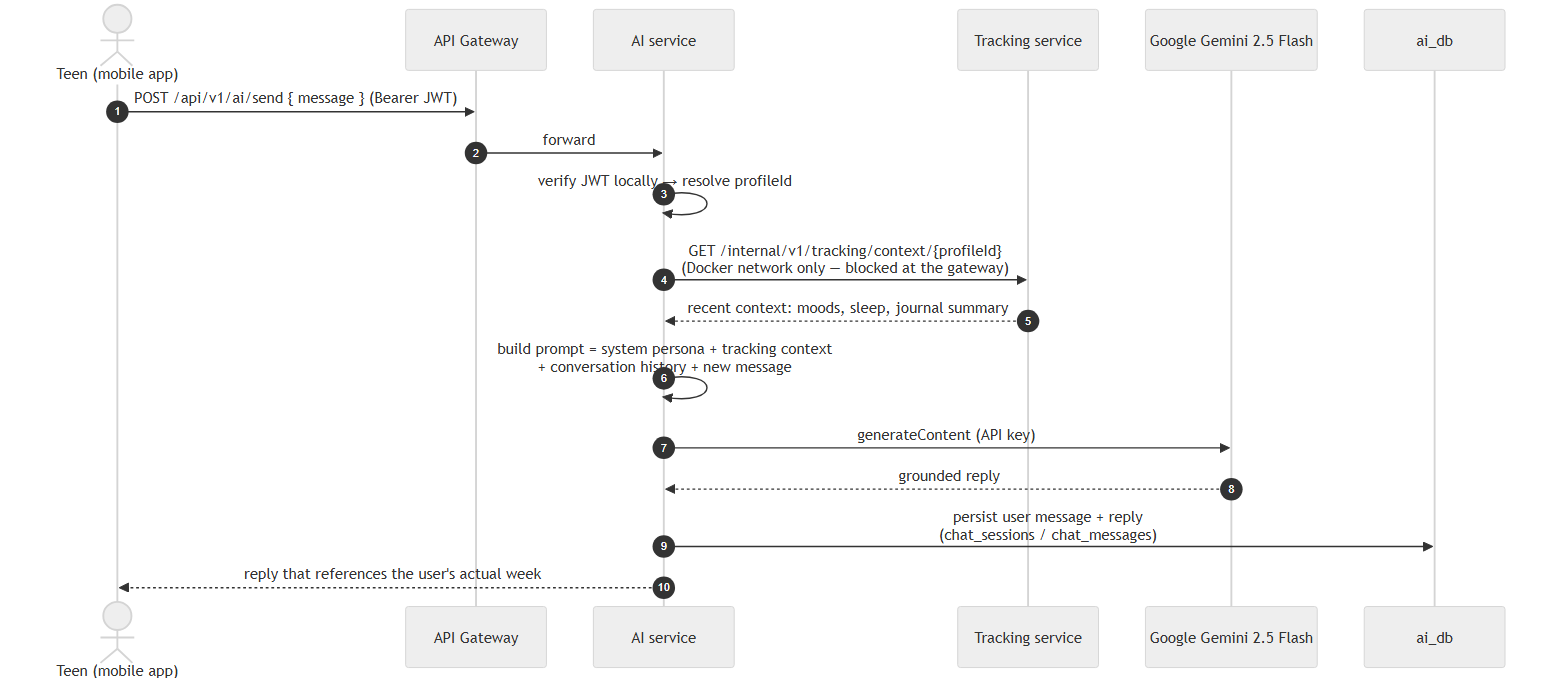
\includegraphics[width=\textwidth]{Chapter3/images/ch3-ai-grounding.png}
    \caption{A sequence diagram of AI grounding}
    \label{fig:ch3-ai-grounding}
\end{figure}

The AI companion is implemented in the AI service. It retrieves the user's recent tracking summary from the Tracking service and includes it as context when calling Google's Gemini 2.5 Flash model~\cite{2024-Gemini-TechReport}. Grounding the model in the user's own data lets the companion respond to something concrete (``you logged trouble sleeping three nights this week'') rather than only offering generic supportive text. Crucially, this retrieval is gated by the same data-access grant model as every other audience (Section~\ref{sec:datasec}): the AI service holds no standing access, and the Tracking service returns context only when the user has an active grant to the reserved AI-companion principal. Consent is off by default --- a user who has not opted in still receives a companion, just one that converses without personal grounding --- and can be revoked at any time from the chat screen, after which the next reply is ungrounded.

Two safeguards run on every message before and around this grounding, and both are deliberately narrow. First, user messages pass a lightweight keyword guardrail: a message matching a small list of Vietnamese self-harm or violence phrases short-circuits the model entirely and returns a fixed response directing the user to emergency hotlines, rather than being sent to Gemini. Second, personally identifying details (emails, phone numbers, and self-introduced names) are scrubbed from the message, history, and context before they leave the platform, and chat contents are encrypted at rest. What the AI service deliberately does not do is any form of clinical risk assessment or automated escalation to a third party --- no scoring, no alerting a therapist or family member --- which is left out of scope, as discussed in Chapter~\ref{Chapter5}, pending the clinical collaboration such a feature would require. The keyword guardrail is a within-conversation safety redirect, not a diagnostic claim.

\section{Professional Workflows}

The Therapist service implements the professional-facing half of the platform: it matches users to therapists based on stated preferences and availability, handles appointment booking, manages Jitsi Meet video consultation sessions~\cite{Jitsi} for the appointment, and stores clinical notes that a therapist records after a session. Appointment booking is a point of particular concern for data integrity, since two concurrent booking requests for the same therapist and time slot must not both succeed; the resolution of this issue is described in Chapter~\ref{Chapter4}.

\section{Peer and Family Connection}
\label{sec:social}

The Social service manages friend relationships and real-time chat over
STOMP/WebSocket. A parent participates through the same mechanism as anyone
else: a parent account (distinguished only by an account type recorded at
registration) connects to their child as a friend, and the connection itself
exposes no tracked data whatsoever.

Visibility is governed exclusively by the grant model of
Section~\ref{sec:datasec}. From a friend's profile screen, a teen may grant
that friend, who is a parent or peer, a scoped access to their tracked data,
issued with a 30-day expiry and revocable at any time; the friend then sees
mood and wellbeing summaries for the granted window, and nothing after
revocation or expiry. There is deliberately no privileged parental path and
no automatic alerting: our baseline study found that an automatic crisis
alert to family was rejected outright as pressure to perform a better mood
than the one being felt, and the professionals we consulted advised that
family connection be explicit and user-controlled. A parent therefore knows
exactly what their child has chosen to show them, which is the point.

\section{Event-Driven Messaging}
\label{sec:events}

\begin{figure}[htbp]
    \centering
    
    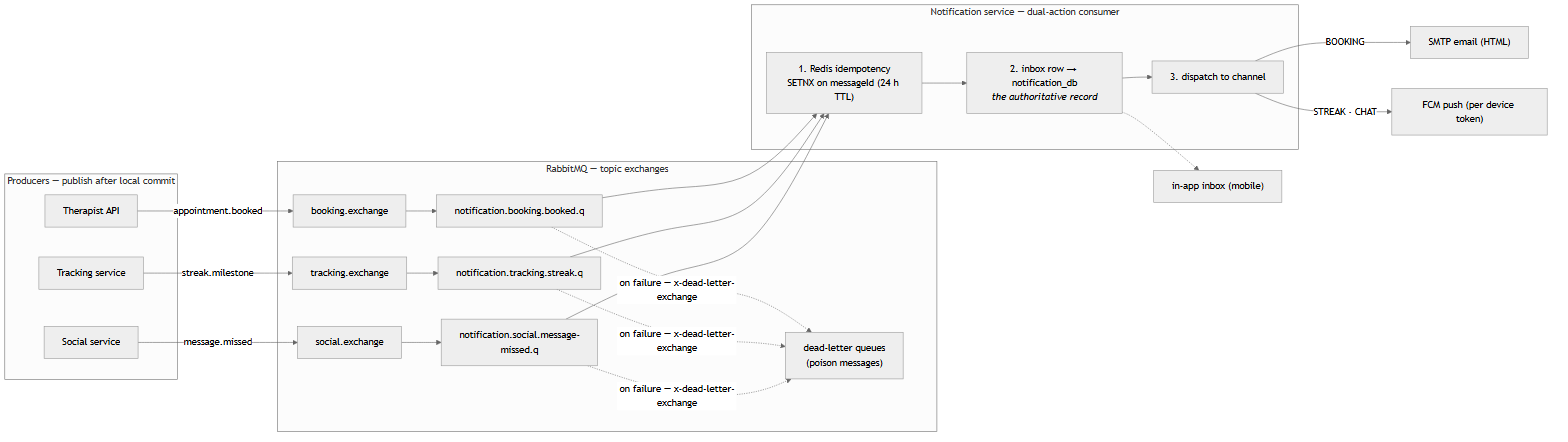
\includegraphics[width=\textwidth]{Chapter3/images/ch3-notification-events.png}
    \caption{An event-flow diagram}
    \label{fig:ch3-notification-events}
\end{figure}

RabbitMQ~\cite{RabbitMQ} connects services that should not depend on each other synchronously. 

Table~\ref{tab:events} catalogs the domain events. Each queue is paired with
a dead-letter queue, so a message that repeatedly fails processing is parked
for inspection rather than blocking the consumer.

\begin{table}[htbp]
  \centering
  \caption{Domain events exchanged over RabbitMQ}
  \label{tab:events}
  % The X columns will automatically expand to fill \textwidth evenly.
  \begin{tabularx}{\textwidth}{|>{\raggedright\arraybackslash}X|l|l|>{\raggedright\arraybackslash}X|}
    \hline
    \textbf{Event} & \textbf{Producer} & \textbf{Consumers} & \textbf{Purpose} \\
    \hline
    \texttt{auth.\allowbreak grant.\allowbreak created}, \texttt{auth.\allowbreak grant.\allowbreak revoked} & Auth &
      Tracking & Replicate consent grants so enforcement is local to the
      data owner \\
    \hline
    \texttt{therapist.\allowbreak profile.\allowbreak updated} & Auth & Therapist &
      Keep the therapist directory in sync with account profiles \\
    \hline
    \texttt{therapist.\allowbreak assignment.\allowbreak changed} & Therapist &
      Social, Auth & Propagate the active patient--therapist assignment
      (e.g.\ opening the corresponding chat) \\
    \hline
    \texttt{appointment.\allowbreak booked} & Therapist & Notification & Fan out booking
      confirmations as push, email, and in-app notifications \\
    
    \hline
  \end{tabularx}
\end{table}

\section{Self-Care Feature Design}
\label{sec:selfcare}

\textbf{Focus Mode.} Check-in prompts are scheduled entirely on the device:
enabling Focus Mode pre-schedules a batch of local notifications at roughly
90-minute intervals (about three days' worth), and the queue is topped up
whenever the application is opened. The Quiet Hours window (22:00--07:00 by
default, user-configurable) is applied at scheduling time and stored only on
the device.

\textbf{Streaks and the mood calendar.} Streaks are computed server-side by
the Tracking service as entries arrive, per tracking category, and the mood
calendar is a read view over the same store. Cross-category trend summaries
shown on the home screen are assembled by the Dashboard service, which reads
Tracking through an internal aggregation API rather than owning any data of
its own.

\textbf{Treasure Box.} Stored positive memories are Tracking-service records
whose photo attachments live in MinIO, and they are surfaced along the
emotion-routing path of Section~\ref{sec:requirements} (FR5): a user logging
sadness is offered their saved memories, a user logging anger a breathing
exercise.

\textbf{Emergency path.} The emergency-support area is a dedicated screen
reachable from anywhere in the application in one tap. It is intentionally
static client-side content, support and hotline resources render.

\section{Deployment Topology}

\begin{figure}[htbp]
    \centering
    
    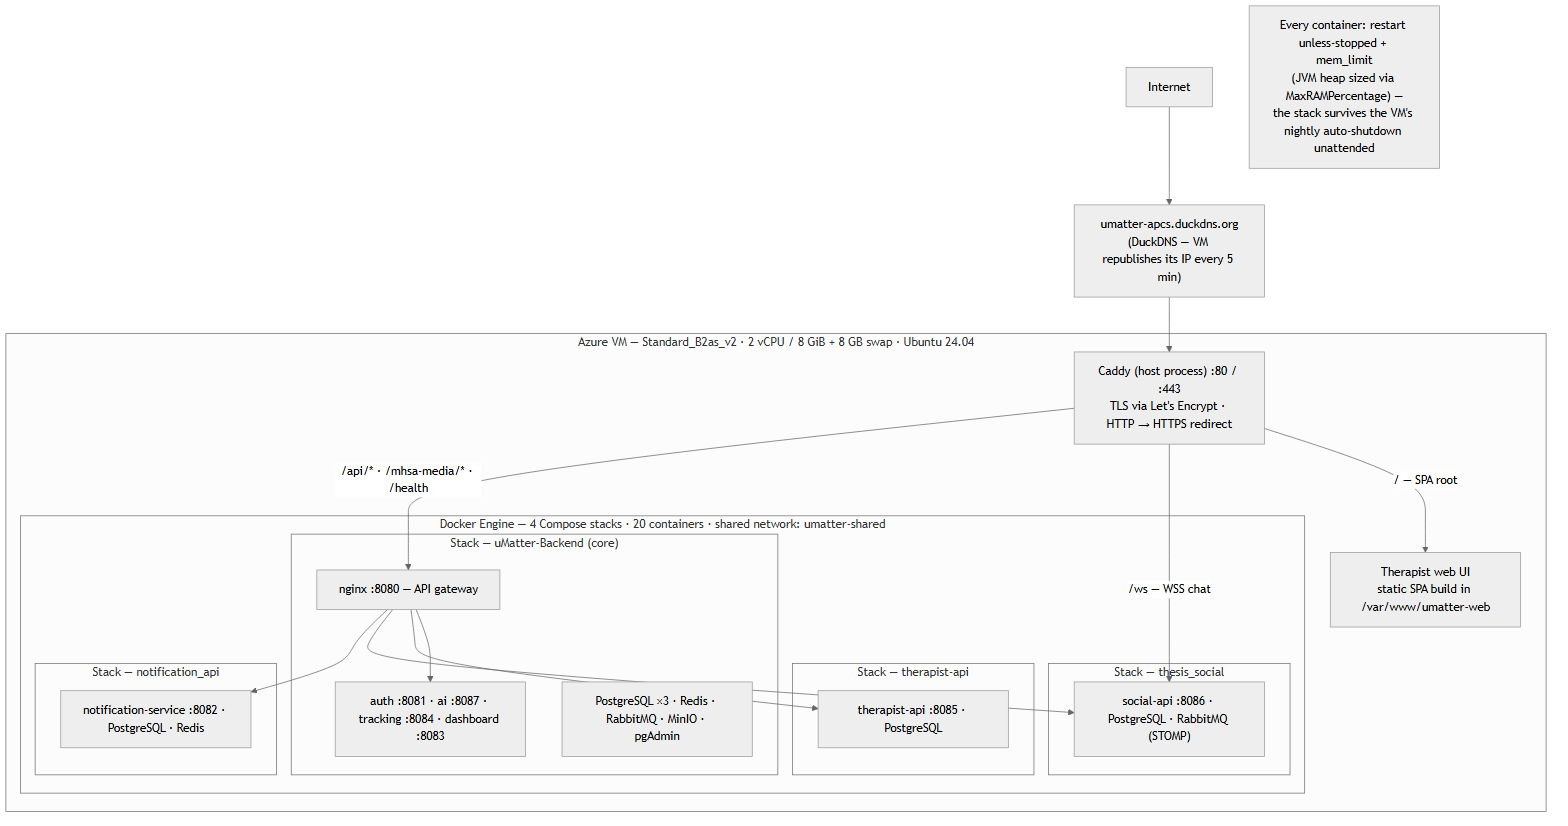
\includegraphics[width=\textwidth]{Chapter3/images/ch3-deployment-topology.png}
    \caption{A deployment diagram}
    \label{fig:ch3-deployment-topology}
\end{figure}

All services are packaged as Docker containers~\cite{Docker} and orchestrated with Docker Compose, grouped into stacks by repository. The full system - Spring Boot services, PostgreSQL instances, RabbitMQ, Redis, MinIO, and supporting tools such as pgAdmin - runs on a single cloud virtual machine, fronted by a reverse proxy that terminates HTTPS. The concrete deployment used for evaluation, including the migration between cloud providers, is described in Chapter~\ref{Chapter4}.
 % System Analysis and Design
\chapter{Implementation and Evaluation}
\label{Chapter4}

This chapter describes the product that the design in Chapter~\ref{Chapter3} became, how it was implemented, the cloud deployment used to run and evaluate it, the distribution of the mobile client, the security-hardening process applied to the platform, and an evaluation of the resulting system. It opens from the user's side, walking the journeys the delivered application actually supports, before turning to the engineering that makes them work.

\section{The Product: End-to-End User Journeys}
\label{sec:product}

Chapters~\ref{Chapter1} to~\ref{Chapter3} argue a problem and specify a design. This section shows what was built, from the position of the person it was built for. The five journeys below are not a feature inventory; they are the paths our trial users actually take, in the order a teenager meets them: the ordinary day first, the hard moment second, and professional care only when the first two are not enough. Each is presented as the sequence of screens a user passes through, and each is annotated with the requirements from Section~\ref{sec:requirements} that it exercises, so that the visual walkthrough and the specification can be read against each other.

Two properties are worth stating before the journeys, because they are what makes the sequences below a single product rather than five separate tools. First, every journey reads from or writes to the same record: the daily entries a user makes in the first journey are what the AI companion, the therapist, and a trusted friend later respond to. Second, no journey crosses a data boundary without the user's explicit act. The consent step is not an afterthought bolted onto the professional journey; it is a screen the user visits deliberately, and the last journey is devoted to it.

\subsection{The daily loop: notice, record, understand}
\label{sec:journey-daily}

\begin{figure}[htbp]
    \centering
    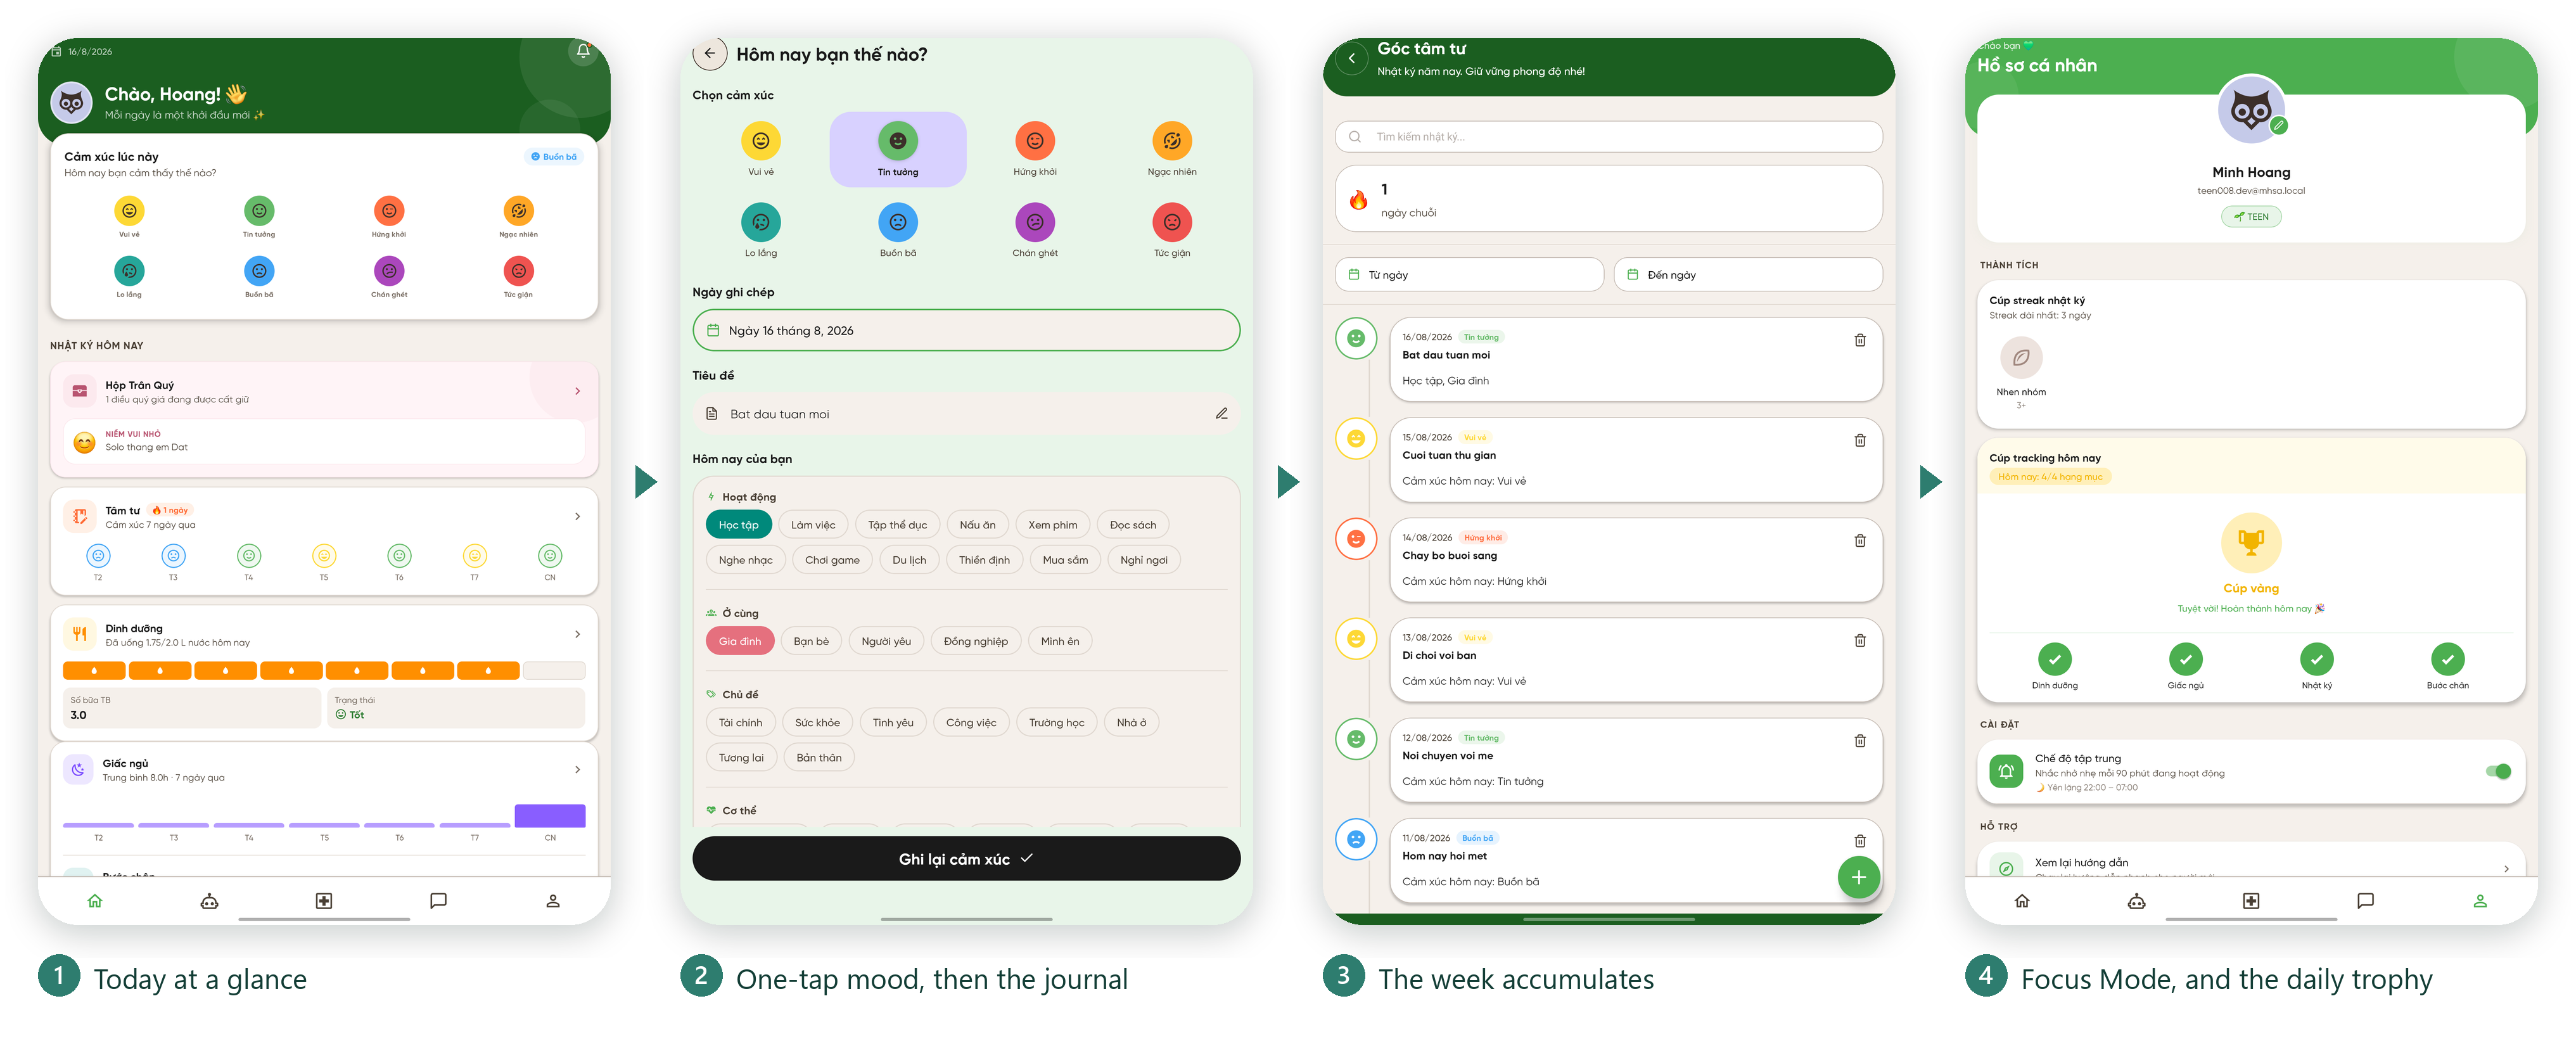
\includegraphics[width=\textwidth]{Chapter4/images/j1-daily-loop.png}
    \caption{The daily loop: a Focus Mode prompt, the mood check-in, the emotional journal, and the trends the entries accumulate into.}
    \label{fig:j1-daily-loop}
\end{figure}

The habit at the centre of the product is a check-in that costs one tap. Figure~\ref{fig:j1-daily-loop} follows it. The application comes to the user rather than waiting to be opened: with Focus Mode enabled, a prompt arrives roughly every ninety minutes through the waking day and falls silent during Quiet Hours, so the recall problem identified in Section~\ref{sec:requirements} is solved without the application becoming a nag (FR3). Acting on the prompt lands the user directly on the check-in, where a mood is chosen and, optionally, a line of context added.

The journal deepens the same act rather than replacing it. A user picks the emotion that fits, names what the day was about, and writes as much or as little as they want, with photographs attached if they help. What the user gets back for this is the fourth screen: a mood calendar that colours each day, per-category streaks, and weekly trends across sleep, steps, nutrition, and breathing (FR1, FR2). This is the return on the habit and the reason it survives past the first week, since the entries stop being data submitted somewhere and become a picture of the user's own month that only they can assemble.

\subsection{The low moment: first aid that is routed, not generic}
\label{sec:journey-low}

\begin{figure}[htbp]
    \centering
    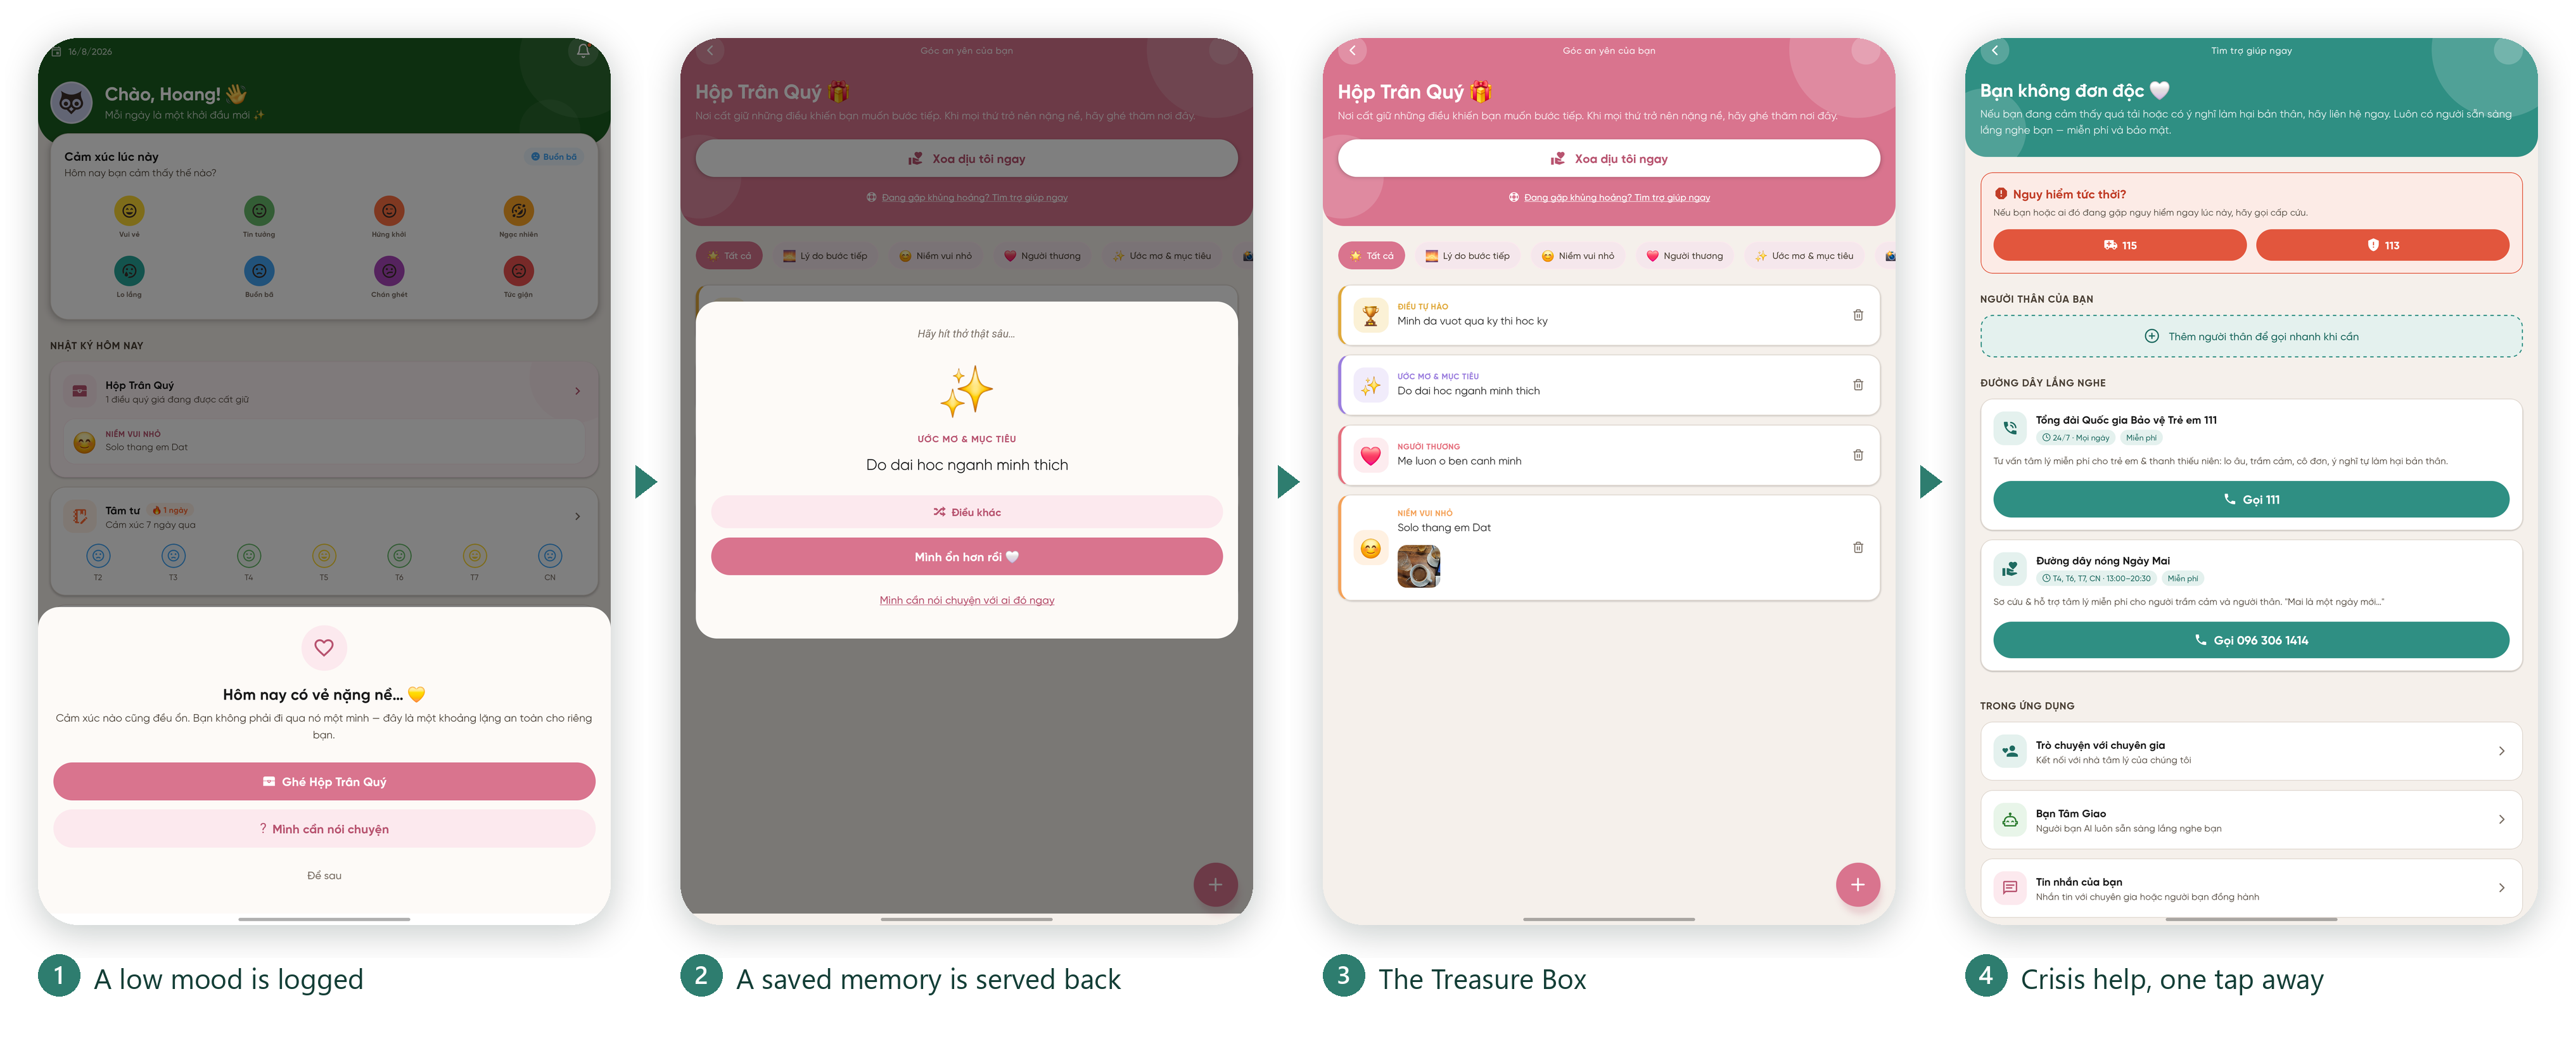
\includegraphics[width=\textwidth]{Chapter4/images/j2-low-moment.png}
    \caption{Logging a negative emotion routes to a matched response: guided breathing for anger, the Treasure Box for sadness, and the emergency area always one tap away.}
    \label{fig:j2-low-moment}
\end{figure}

The design decision that most distinguishes the product is what happens immediately after a negative mood is logged. The application does not return the user to a dashboard. It routes them, and it routes by which emotion was recorded, following the guidance of the professionals consulted in Section~\ref{sec:elicitation}: anger is met with a guided breathing exercise, sadness with the user's own Treasure Box (FR5).

The Treasure Box, shown in the third panel of Figure~\ref{fig:j2-low-moment}, is the feature trial users valued most (Section~\ref{sec:most-valued}). Its premise is that a low mood makes good memories hard to reach, so the memories are saved in advance, on a good day, and reopened on the bad one: photographs, kind messages, small wins, and reasons to keep going, put somewhere the user can find them at the moment recall fails. Running alongside both paths, the emergency area is reachable in one tap from anywhere in the application and renders entirely from client-side content, so it stays available even when the backend is not (FR5).

\subsection{Someone to talk to, at any hour}
\label{sec:journey-companion}

\begin{figure}[htbp]
    \centering
    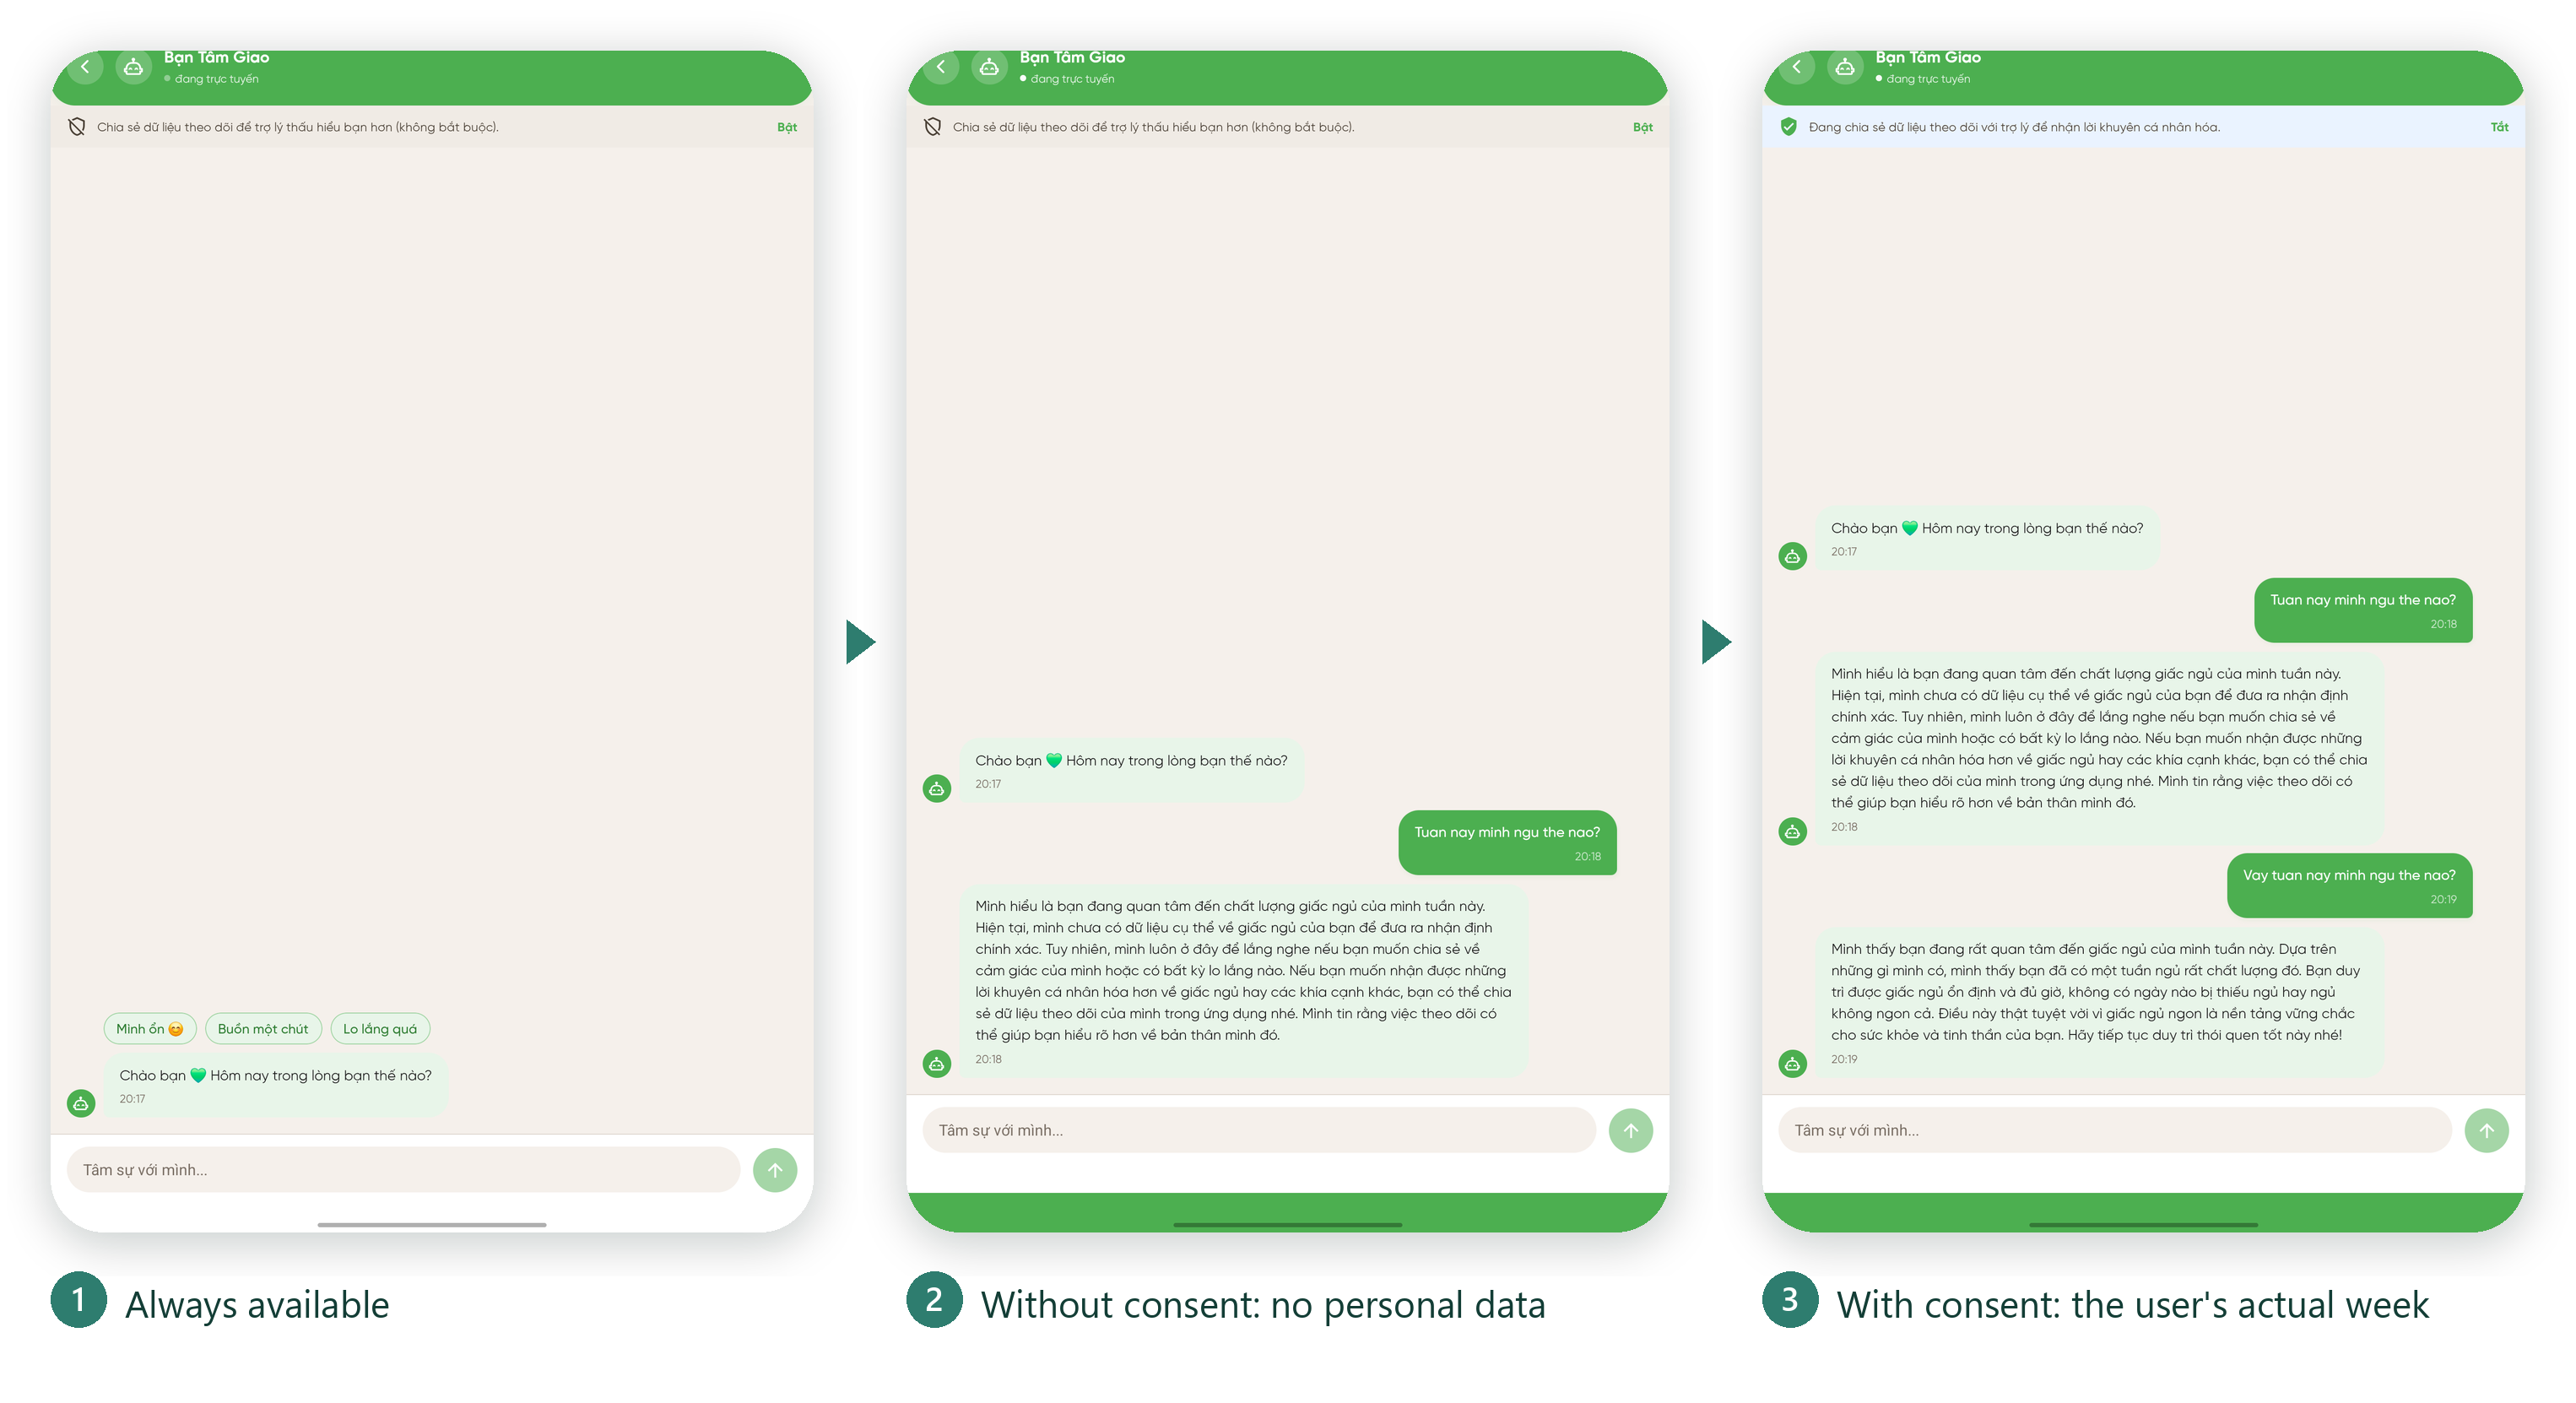
\includegraphics[width=\textwidth]{Chapter4/images/j3-companion.png}
    \caption{B\d{a}n T\^am Giao: an always-available companion whose replies draw on the user's own week when, and only when, access has been granted.}
    \label{fig:j3-companion}
\end{figure}

Trial users reported reaching for the companion late at night, when contacting a friend or a therapist was not an option. That availability is the feature. What separates it from a general-purpose chatbot is that it can be given the user's own recent history, so a reply can respond to a week that actually happened rather than to nothing at all (FR4). The grounding is opt-in and off by default: a user who never grants access still gets a companion, just one without personal context, and the difference between the two is visible in the replies themselves.

The contrast is visible directly in Figure~\ref{fig:j3-companion}: asked the same question twice, the companion first states plainly that it has no sleep data and invites the user to share it, and then, once the grant is switched on in the banner at the top of the conversation, characterizes the week from the user's actual logs. The grounding is nevertheless qualitative rather than numeric, for the reasons set out in Section~\ref{sec:expert-findings}.

The safety behaviour is deliberately narrow. A message matching a small list of self-harm or violence phrases bypasses the model entirely and returns the crisis hotlines directly. This is a within-conversation redirect and not a clinical assessment; the system performs no risk scoring and raises no automated alert to any third party, for the reasons set out in Chapter~\ref{Chapter5}.

\subsection{Crossing into professional care}
\label{sec:journey-professional}

\begin{figure}[htbp]
    \centering
    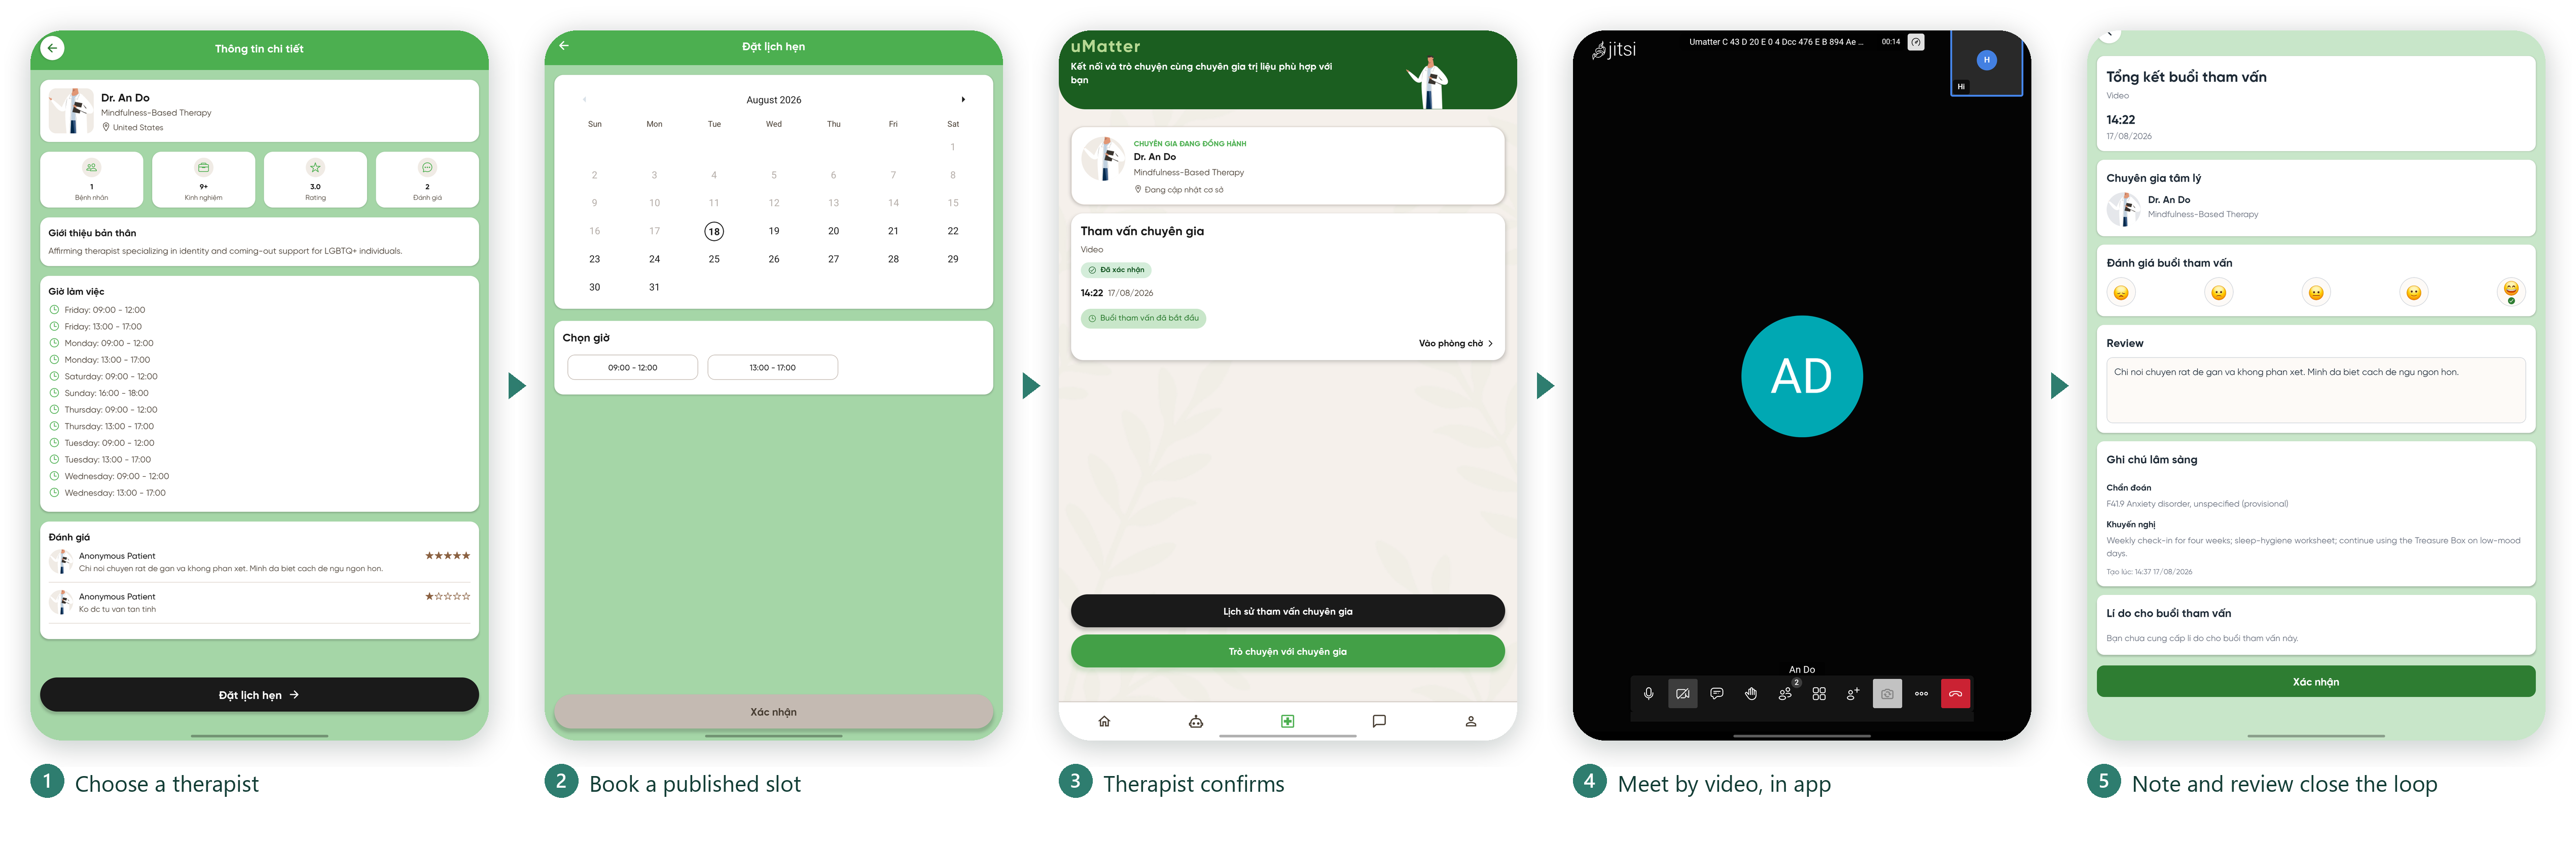
\includegraphics[width=\textwidth]{Chapter4/images/j4-professional.png}
    \caption{From choosing a therapist to sitting in the consultation, without leaving the application.}
    \label{fig:j4-professional}
\end{figure}

When self-help is not enough, the crossing into professional care happens inside the same application. A short intake form asks what the user is going through, how they prefer to be met, and whether prior therapy has been tried, and ranks therapists by the overlap with what each one treats (FR6). Booking is a slot on the therapist's published calendar; confirmation arrives as a push notification and an email so the appointment does not slip past (FR8). The session runs as video inside the application, and afterwards the user reads the therapist's structured note and leaves a review.

Figure~\ref{fig:j4-professional} follows one appointment through that arc. The therapist's profile states what they treat and when they work; the calendar exposes only the slots they have actually published; the appointment then waits, visibly, until the therapist accepts it. The video room opens ten minutes before the hour and no earlier, and the user who arrives first waits in a lobby rather than in an empty room --- the session cannot begin until the therapist is present. The final panel is where the loop closes: the therapist's finalized note, its diagnosis and its recommendations, is presented to the user on the same screen that asks them to rate the session, so reading what the professional concluded and giving feedback on it are a single act rather than two.

The therapist works the other side of the same appointment from the web dashboard described in Section~\ref{sec:professional}. This is the point at which the black box between sessions closes: a therapist who has been granted access opens the consultation already knowing how the patient's month went, instead of spending the first part of the session reconstructing it from memory.

\subsection{Choosing who sees}
\label{sec:journey-consent}

\begin{figure}[htbp]
    \centering
    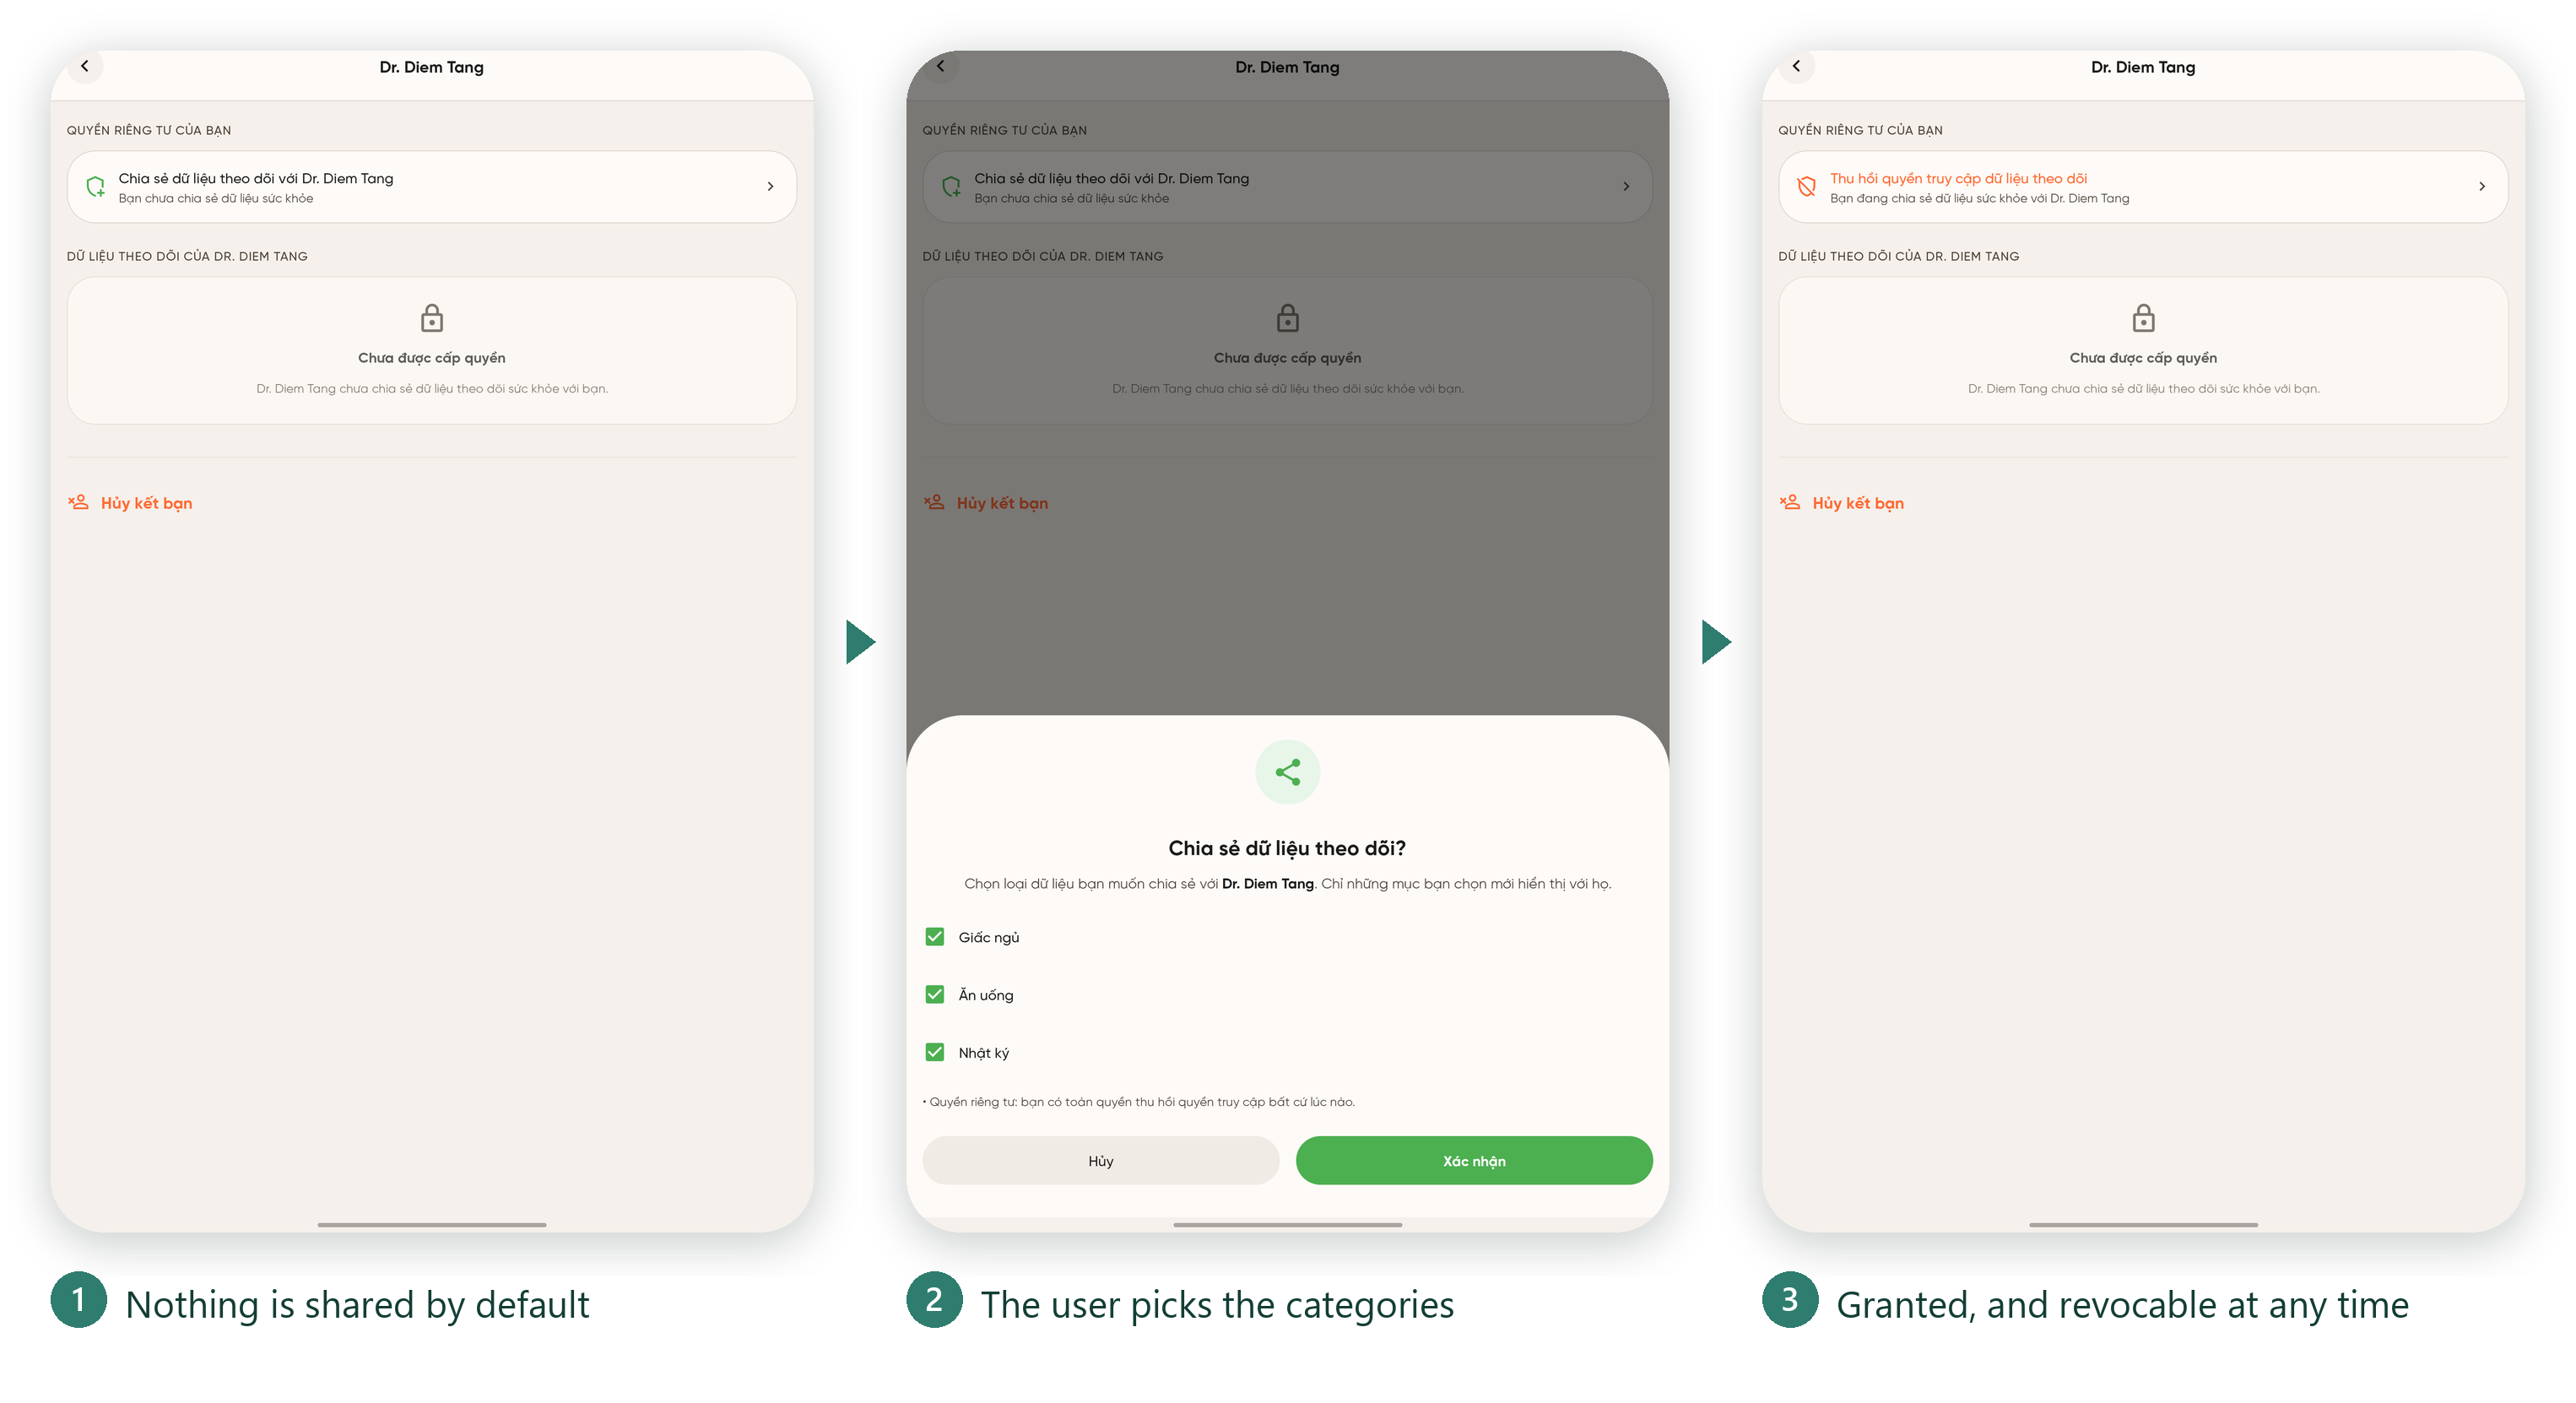
\includegraphics[width=\textwidth]{Chapter4/images/j5-consent.png}
    \caption{One consent mechanism for every audience: nothing is shared until the user selects the categories to expose, and the grant is revocable from the same screen afterwards.}
    \label{fig:j5-consent}
\end{figure}

The final journey is the one that makes the other four safe to use, and trial users identified it as the precondition for writing honestly at all (Section~\ref{sec:expert-findings}). Nothing a user records is visible to anyone by default, and Figure~\ref{fig:j5-consent} follows the grant from that default to an active, revocable share. The screen opens stating plainly that nothing has been shared; the user then chooses which categories of their record to expose, category by category, and confirms. Afterwards the same row inverts into a revoke control, so withdrawing access is exactly as easy as granting it (FR1, FR6, FR7, NFR1). The grant is surfaced wherever the audience appears rather than buried in a settings menu: the banner at the top of the AI conversation in Figure~\ref{fig:j3-companion} is the companion's own grant control, carrying the same meaning and the same server-side enforcement as the grant a user extends to a therapist or a friend.

The point is that this screen is the only way in, for every audience. A therapist, a parent, a friend, and the AI companion are grantees of exactly the same mechanism, enforced server-side. There is deliberately no privileged parental path and no automatic alerting: our baseline study found that automatic crisis alerts to family were rejected as pressure to perform a better mood than the one being felt. A parent therefore sees precisely what their child chose to show them, which is the intended outcome rather than a limitation.

\subsection{What the journeys share}

Table~\ref{tab:journeys} maps each journey to the requirements it exercises. Read together, the journeys are one loop rather than five features: the daily record made in the first is what the second routes on, what the third grounds its replies in, what the fourth gives a therapist to work from, and what the fifth governs access to. This is the unification argued for in Chapter~\ref{Chapter1}, expressed as the path a user walks rather than as a component diagram, and it is the reason a single platform was worth building instead of assembling the same capabilities from four separate products.

\begin{table}[htbp]
  \centering
  \caption{User journeys and the requirements they exercise}
  \label{tab:journeys}
  \begin{tabular}{|l|p{7.4cm}|l|}
    \hline
    \textbf{Journey} & \textbf{What the user does} & \textbf{Req.} \\
    \hline
    Daily loop & Responds to a Focus Mode prompt, logs a mood, writes a
                 journal entry, reads back the week. & FR1--FR3 \\
    \hline
    Low moment & Logs a negative emotion and is routed to breathing, the
                 Treasure Box, or the emergency area. & FR5 \\
    \hline
    Companion & Talks to the AI at any hour, optionally grounded in their
                own record. & FR4 \\
    \hline
    Professional & Completes intake, books a slot, attends by video, reads
                   the note, leaves a review. & FR6, FR8 \\
    \hline
    Consent & Grants scoped access to a therapist, parent, friend, or the
              companion, and revokes it. & FR7, NFR1 \\
    \hline
  \end{tabular}
\end{table}

\section{Implementation Overview}

The backend services are implemented in Java 17. The Auth, Tracking, AI, and Dashboard services are built on Spring Boot~4.0 and organized as a Maven multi-module project so that shared code (for example, JWT validation logic) is written once and reused. The Therapist service is a separate Gradle project on Spring Boot~4.0, while the Social and Notification services are Gradle projects on the slightly earlier Spring Boot~3.3, reflecting when they were added to the system. Persistence throughout uses Spring Data JPA over PostgreSQL. The Social service's real-time chat is implemented with STOMP over WebSocket, and the Notification service integrates Firebase Cloud Messaging for push delivery in addition to email and an in-app inbox.

On the client side, the mobile application for teenagers is built with React Native~0.83 and React~19 in TypeScript, and the therapist-facing web dashboard is built with React~18, TypeScript, Vite, and Tailwind CSS. Appendix~\ref{Appendix5} records why these platforms, the database, and the language model behind the AI companion were preferred to the alternatives considered.

\section{Deployment}

uMatter was originally deployed on Oracle Cloud Infrastructure (OCI). During the course of this thesis, the deployment was migrated in full to Microsoft Azure, under an Azure for Students subscription. The migration involved:

\begin{itemize}
\item Resolving Azure region-policy restrictions that initially blocked the target subscription from provisioning a virtual machine in the desired region.
\item Configuring Network Security Group (NSG) rules to open the ports required by the API gateway and by directly-exposed services (for example, RabbitMQ's management port during setup, and ports 80 and 443 for the reverse proxy).
\item Working around Azure Cloud Shell setup issues encountered while preparing the target VM.
\item Reproducing the auto-shutdown behavior available on the previous provider using Azure's built-in scheduled auto-shutdown, to control cost under the student subscription, with the containers configured to restart automatically on boot so they come back up automatically when the VM is next started.
\end{itemize}

The resulting deployment runs on a single, right-sized Azure VM hosting 20 containers: multiple Spring Boot JVM services, several PostgreSQL instances (one per owning service), RabbitMQ, Redis, MinIO, and pgAdmin. HTTPS routing is provided by Caddy as a reverse proxy, with DuckDNS supplying a stable hostname for the VM's dynamic address, and the VM's public IP configured as static so the hostname does not need to be re-pointed after the nightly auto-shutdown cycle. This mirrors the general topology described in Chapter~\ref{Chapter3}, with Caddy taking the reverse-proxy/HTTPS-termination role and Nginx continuing to serve as the internal API gateway between the proxy and the backend services.

\subsection{Mobile Application Distribution}

The mobile client for teenagers/patients was packaged and published to the Google Play Store, rather than distributed as a manually installed APK. Publishing through Google Play means end users install and update the app the same way as any other Android application, without needing to trust or manually side-load a build shared outside the store.

This distribution choice also shaped a concrete backend requirement: the published app communicates with the API gateway exclusively over HTTPS on port 443, because modern Android builds block plaintext HTTP traffic by default. Terminating TLS correctly at the reverse proxy, using a Let's Encrypt certificate obtained over port 80, was therefore not an optional hardening step but a hard prerequisite for the Play Store build to reach the backend at all. This is why ports 80 and 443 were treated as non-negotiable when the NSG rules were configured.

\section{Security Hardening}

Because uMatter handles sensitive personal data and coordinates real appointments, the implemented services were subjected to structured security audits organized around the OWASP Top~10 risk categories~\cite{2021-OWASP-Top10}, covering three areas in particular:

\begin{itemize}
\item \textbf{Business logic correctness}: verifying that workflows such as matching, booking, and permission granting behave correctly under normal and adversarial input, not only in the happy path.
\item \textbf{Access control}: specifically JPQL injection patterns in hand-written queries, insecure direct object references (for example, a user supplying another user's record identifier to an endpoint that does not re-check ownership), and mass assignment (a client supplying extra fields in a request body that get bound to fields the client should not be able to set, such as a role or a permission flag).
\item \textbf{Data integrity}: ensuring that concurrent requests cannot leave the system in an inconsistent state.
\end{itemize}

The most significant data-integrity issue identified was a race condition in appointment booking: two concurrent requests to book the same therapist for the same time slot could both pass an application-level availability check before either write was committed, resulting in a double booking. This was closed not by adding an application-level lock, which would not be safe against multiple service instances, but by making the slot claim a single atomic database operation: booking a slot is a conditional update that sets the slot's booked flag to true only where it is still false, so exactly one of two concurrent requests updates a row and the other is rejected. A unique constraint on the appointment's slot reference backs this up as a second line of defense. Because the guarantee lives in the database itself, it holds regardless of how many instances of the Therapist service are running concurrently.

The most significant access-control finding was in the AI service's own path to a user's tracking data, rather than in a caller manipulating another user's identifier. The Tracking service's internal context endpoint, used by the AI service to retrieve grounding data, was reachable by any authenticated internal caller. It performed no check that the caller had actually been granted access to that data, relying instead on network-level trust between services. This is precisely the class of implicit trust that the permission-based data-sharing model in Section~\ref{sec:datasec} is designed to remove. The fix followed the same pattern used elsewhere in the codebase: the AI companion was added as a reserved grantee in the existing access-grant table, and the context endpoint now checks for an active grant before returning anything, exactly as it already did for a therapist. No new authorization mechanism was introduced; an existing one was extended to a caller that had previously been exempted from it.

\section{Evaluation}

The system was evaluated along several dimensions: functional completeness against the design goals in Chapter~\ref{Chapter1}, security posture after hardening, feature positioning relative to the competitive landscape reviewed in Chapter~\ref{Chapter2}, and qualitative feedback from trial users and mental-health professionals, including the features they valued most and the wider findings that emerged from the design, trial, and consultation process.

\subsection{Functional Completeness}
\label{sec:functional-completeness}

All seven backend services described in Chapter~\ref{Chapter3} are implemented and deployed, and both client applications (mobile for teens, web for therapists) are functional against them. Table~\ref{tab:traceability} in Appendix~\ref{Appendix3} traces each requirement from Section~\ref{sec:requirements} to its implementation status.

Every requirement is met except FR8: all three notification channels (push, email, and the in-app inbox) work and fire end-to-end for appointment booking, but the other domain events intended to raise notifications are not currently wired to producers, so coverage across events is partial.

\subsection{Security Posture}

The structured audits identified and closed concrete issues in each of the three areas examined (business logic, access control, and data integrity), including the appointment-booking race condition described above. This does not constitute a formal, independent penetration test, and should be read as an internal hardening pass rather than a certification of the system's security; further external review would be a reasonable next step before any production use involving real users.

\subsection{Comparison with Existing Platforms}

Revisiting the comparison in Table~\ref{tab:competitive}, the implemented system delivers on the feature combination that motivated this thesis: self-care tracking, an AI companion grounded in the user's own data, and peer social features, alongside licensed-therapist matching, booking, video consultation, and clinical notes, connected by a permission-based sharing model that none of the compared single-purpose platforms offer in combination. The clearest gap relative to mature commercial platforms such as BetterHelp and Talkspace~\cite{BetterHelp,Talkspace} is operational maturity: those platforms have been hardened and scaled in production for years, whereas uMatter, as a thesis project, has been validated on a single-VM deployment and an internal security-audit process rather than at production scale.

\subsection{Most-Valued Features}
\label{sec:most-valued}

\subsubsection{The Treasure Box (Hộp Trân Quý)}

The Treasure Box is a personal store of positive ``core memories'' (photos, kind messages, small wins, life goals, and motivating reflections) that a user saves ahead of time and reopens whenever they need comforting. On a low day, when negative bias makes good memories hard to recall, this pre-saved anchor gives users self-compassion they can reach for exactly when they need it. The feature grew directly out of expert collaboration: Miss Pham Thi Thanh Qui first suggested reconnecting users with their reasons for living when feeling low, and mister Vuong Nguyen Toan Thien, CEO of LUMOS, concretized that idea into the Treasure Box, grounding it in research on positive memory and mood. Within the app it is one destination in uMatter's ``psychology first-aid'' response to a low mood, alongside guided breathing and the SOS crisis contacts.

\subsubsection{Daily Reflective Tracking}

Daily reflective tracking is the everyday self-check-in habit at the heart of the app: mood check-ins, the emotional journal, logs for sleep, nutrition, and water, automatic step counting, and guided breathing, each surfaced as a friendly ``today'' card with weekly trends. Doctor Pham Tran Thanh Nghiep assessed these features as ``already very good'' and helpful to users' mental wellbeing, and Miss Qui, holding that physical and mental health are inseparable, endorsed the physical-health tracking (steps, sleep, nutrition, breathing) as a legitimate mental-health signal. Gentle Focus-Mode reminders roughly every ninety minutes, daily achievement ``trophies'' for a completed chain of self-care tasks, and streaks keep it a low-friction habit rather than a chore. The same daily data also grounds the AI companion, the therapist's view (under permission), and the trusted-friend view, so the feature most valued on its own is also what makes the rest of the platform work.

\subsection{Key Findings}
\label{sec:expert-findings}

\subsubsection{Findings from the Design and Development Process}

% TODO: viết lại. Ý chính (rút ra từ Chapter 3 & 4):
\begin{itemize}
\item \textbf{A weekly review cycle kept the feature set close to what users actually asked for.} Development was never carried out in isolation from the people it was for: each phase closed with a meeting held either with the mental-health professionals or with the trial users, and with weekly supervision from the advisor, so a proposed function was argued for, built, and then judged by someone outside the team within the same phase (Section~\ref{sec:elicitation}, Appendix~\ref{Appendix6}). The cost is visible as features removed rather than added, which is the point: the surveys below were dropped, and the Treasure Box was added, because the review said so rather than because the team preferred it.

\item \textbf{Unifying self-care and therapy is feasible behind one permission model.} A single microservices platform can serve both halves of the care journey without merging the data, as long as sharing is explicit, granular, and revocable.
\item \textbf{Network-level trust between services is not enough.} The most instructive security finding was that an internal caller (the AI service) could reach a user's tracking data with no explicit grant, meaning that implicit inter-service trust is exactly the class of assumption the permission model must remove, even for internal callers.
\item \textbf{Grounding the AI in the user's own data}, with a safe fallback, is what makes it useful without over-reaching. Toggling the grant changes the companion's replies materially: without it the AI states plainly that it has no tracking data, while with it the same question draws a reply reflecting the user's actual sleep, mood, and nutrition patterns. The grounding is nevertheless \emph{qualitative}. The companion characterizes the week (``your sleep has not been deep or long enough'') but never quotes a figure, even when explicitly asked for one. Two deliberate choices produce this: the system prompt forbids reciting the context mechanically, to keep the tone conversational rather than clinical, and the context passed to the model is itself an aggregate summary (an average, a count of poor nights, a set of mood tags) carrying no per-day values or dates. The companion is therefore demonstrably personalized but not \emph{verifiable}: a user cannot check a reply against the numbers they logged.
% \item \textbf{[placeholder]} % TODO: thêm finding kỹ thuật khác nếu cần.
\end{itemize}

\subsubsection{Findings from User Feedback}

The findings below come from the seven trial users listed in Appendix~\ref{Appendix6}: they were interviewed for user stories before implementation began and re-interviewed against the working build as each development phase closed, in semi-structured sessions held roughly monthly, alternating with the expert consultations. A separate cohort of seventeen testers exercised the published Android build over the fourteen-day Google Play closed-testing period; that cohort reported defects rather than design opinions, and its output is release-phase testing rather than user research. The trial group is small and drawn from the team's own circle, so what follows is qualitative and carries no statistical weight.

\begin{itemize}
\item \textbf{Daily journaling beats periodic surveys.} Trial users found the weekly/monthly surveys redundant next to the daily journal and 3-hourly mood check-ins; the surveys were dropped.
\item \textbf{The most-loved features were the Treasure Box and daily tracking} (Section~\ref{sec:most-valued}).
\item \textbf{The consent gate is what made honest journaling possible.} Users reported writing honestly in the emotional journal only once they understood that a therapist or a trusted friend sees nothing without an explicit grant that they can revoke at any time. 
\item \textbf{The AI companion was valued for availability, yet the efficiency of the interaction needs improvement.} Users reached for the companion late at night, when contacting a friend or a therapist was not an option. However, the companion's replies is too vague and inefficient and barely reflective of user's actual data even when grounded, making it far inferior to a stronger Gemini or ChatGPT model without a any previous context. 
\end{itemize}

\subsubsection{Findings from Expert Consultations}

\begin{itemize}
\item \textbf{Miss Qui} endorsed the option-based emotional journal, the gentle 3-hourly mood check-ins (for complete, meaningful data and for helping users pay attention to themselves), the 4-7-8 breathing exercise as a response to anger, the reward/trophy loop for completing a chain of self-care tasks, the revocable trusted-person sharing, and physical-health tracking such as steps.
\item \textbf{Mister Thien} praised the Treasure Box concept, the emotion timeline for complete mental-health data, the ``psychology first-aid'' bundle for negative moods (breathing, SOS contact, Treasure Box), and the SOS hotline page.
\item \textbf{Doctor Nghiep} gave the strongest endorsement of the daily reflective tracking features (``already very good'').
\end{itemize}
 % Implementation and Evaluation
\chapter{Conclusion and Future Work}
\label{Chapter5}

\section{Conclusion}

This thesis set out to design, implement, and evaluate uMatter, a mental-health support platform for teenagers that unifies self-care tracking with professional therapy access, addressing a gap identified between existing self-care applications (Daylio, Bearable) and existing therapy platforms (BetterHelp, Talkspace, Wysa), none of which combine both halves of the care journey behind a single, permission-based data-sharing model.

The resulting system is a seven-service microservices architecture behind an API gateway, with a database-per-service data layer, stateless JWT authentication, and an AI companion grounded in each user's own tracking data. A structured security-hardening process identified and resolved concrete issues across business logic, access control, and data integrity, including a database-level fix for a race condition in appointment booking. The full stack was deployed to cloud infrastructure - migrated from Oracle Cloud to Microsoft Azure over the course of the project - and evaluated both functionally and against the competitive landscape it was designed to improve on.

Taken together, this work shows that a single, security-conscious microservices platform can plausibly serve both sides of adolescent mental health support - self-care and professional therapy - rather than requiring a teenager to use two disconnected products.

% =====================================================================
% NEW SECTION (skeleton) - các feature được đánh giá cao bởi người dùng
% và chuyên gia. Draft tiếng Anh + placeholder; về nhà viết lại kỹ hơn.
% =====================================================================
\section{Features Most Valued by Users and Experts}

Across the user trials and the three expert consultations conducted during this project (Section~\ref{sec:expert-findings}), two parts of uMatter stood out as the most consistently and highly valued: the \textbf{Treasure Box (Hộp Trân Quý)} and the suite of \textbf{daily reflective tracking} features. Both are described in the product tour in Appendix~\ref{...} % TODO: trỏ tới appendix/showcase phù hợp
and are singled out here because they attracted the strongest positive response.

\subsection{The Treasure Box (Hộp Trân Quý)}

% TODO: viết lại thành đoạn văn hoàn chỉnh. Ý chính:
\begin{itemize}
\item \textbf{What it is.} A personal store of positive ``core memories'' - photos, kind messages, small wins, life goals, and motivating reflections - that a user saves ahead of time and reopens whenever they need comforting.
\item \textbf{Why it was valued.} On a low day, negative bias makes good memories hard to recall; a pre-saved, reliable anchor back to the good gives users self-compassion they can reach for exactly when they need it.
\item \textbf{Where it came from.} The feature grew directly out of expert collaboration: Miss Pham Thi Thanh Qui first suggested a feature to reconnect users with their reasons for living and their motivation when feeling low, and mister Vuong Nguyen Toan Thien, the CEO of LUMOS, concretized that idea into the Treasure Box, grounding it in psychological research on positive memory and mood.
\item \textbf{How it fits.} It is one of the destinations in uMatter's ``psychology first-aid'' response to a negative mood, alongside guided breathing and the SOS crisis contacts.
\item \textbf{[placeholder]} % TODO: chèn phản hồi/đánh giá cụ thể của người dùng thử (trích dẫn, số liệu nếu có).
\end{itemize}

\subsection{Daily Reflective Tracking}

% TODO: viết lại thành đoạn văn hoàn chỉnh. Ý chính:
\begin{itemize}
\item \textbf{What it is.} The everyday self-check-in habit at the heart of the app: mood check-ins, the emotional journal, sleep, nutrition and water, automatic step counting, and guided breathing - each surfaced as a friendly ``today'' card with weekly trends.
\item \textbf{Why it was valued.} Docter Pham Tran Thanh Nghiep assessed the daily reflective tracking features as ``already very good'' and already helpful to users' mental wellbeing. Miss Qui emphasised that physical and mental health are inseparable, endorsing the physical-health tracking (steps, sleep, nutrition, breathing) as legitimate mental-health signal.
\item \textbf{What makes it stick.} Gentle Focus-Mode reminders roughly every ninety minutes, daily achievement ``trophies'' for completing a chain of self-care tasks, and streaks turn tracking into a low-friction daily habit rather than a chore.
\item \textbf{Why it matters system-wide.} This daily data is also the foundation that grounds the AI companion, the therapist's view (under permission), and the trusted-friend view - so the feature most valued on its own is also what makes the rest of the platform work.
\item \textbf{[placeholder]} % TODO: chèn phản hồi/đánh giá cụ thể của người dùng thử.
\end{itemize}

% =====================================================================
% NEW SECTION (skeleton) - Findings: từ quá trình làm thesis,
% từ phản hồi người dùng, và từ 3 chuyên gia tâm lý.
% =====================================================================
\section{Key Findings}
\label{sec:expert-findings}

Beyond the system itself, the design, trial, and consultation process surfaced a number of findings worth stating explicitly. % TODO: câu mở đầu, viết lại cho mượt.

\subsection{Findings from the Design and Development Process}

% TODO: viết lại. Ý chính (rút ra từ Chapter 3 & 4):
\begin{itemize}
\item \textbf{Unifying self-care and therapy is feasible behind one permission model.} A single microservices platform can serve both halves of the care journey without merging the data, as long as sharing is explicit, granular, and revocable.
\item \textbf{Network-level trust between services is not enough.} The most instructive security finding was that an internal caller (the AI service) could reach a user's tracking data with no explicit grant - implicit inter-service trust is exactly the class of assumption the permission model must remove, even for internal callers.
\item \textbf{Grounding the AI in the user's own data, with a safe fallback, is what makes it useful without over-reaching.} % TODO: mở rộng nếu muốn.
\item \textbf{[placeholder]} % TODO: thêm finding kỹ thuật khác nếu cần.
\end{itemize}

\subsection{Findings from User Feedback}

% TODO: viết lại. Cần điền số người dùng thử / phương pháp khảo sát.
\begin{itemize}
\item \textbf{Daily journaling beats periodic surveys.} Trial users found the weekly/monthly surveys redundant next to the daily journal and 3-hourly mood check-ins; the surveys were dropped. Finding: high-frequency, low-friction daily logging yields richer and more meaningful data than periodic questionnaires.
\item \textbf{The most-loved features were the Treasure Box and daily tracking} (Section~\ref{...}), % TODO: cross-ref section trên
which is why they are highlighted separately above.
\item \textbf{[placeholder]} % TODO: điền các phản hồi khác của người dùng thử, số liệu đánh giá, trích dẫn. Mô tả cỡ mẫu và cách khảo sát (N người dùng thử, thời gian).
\end{itemize}

\subsection{Findings from Expert Consultations}

We consulted three mental-health professionals during the project: % TODO: có thể chuyển thành bảng.
\begin{itemize}
\item \textbf{Miss Pham Thi Thanh Qui} - counsellor, Psychological Counselling Office, University of Science, VNU-HCM (in person, 29 May 2026).
\item \textbf{Mister Vuong Nguyen Toan Thien} - CEO, LUMOS (online, 2 June 2026).
\item \textbf{Doctor Pham Tran Thanh Nghiep} - physician, Hoan My Sai Gon Hospital (online, 3 June 2026).
\end{itemize}

\noindent\textbf{What the experts validated and praised.} % TODO: viết lại thành văn.
\begin{itemize}
\item \textbf{Miss Qui} endorsed the option-based emotional journal, the gentle 3-hourly mood check-ins (for complete, meaningful data and for helping users pay attention to themselves), the 4-7-8 breathing exercise as a response to anger, the reward/trophy loop for completing a chain of self-care tasks, the revocable trusted-person sharing, and physical-health tracking such as steps.
\item \textbf{Mister Thien} contributed and praised the Treasure Box concept, the emotion timeline for complete mental-health data, the ``psychology first-aid'' bundle for negative moods (breathing, SOS contact, Treasure Box), and the SOS hotline page.
\item \textbf{Doctor Nghiep} gave the strongest endorsement of the daily reflective tracking features (``already very good'') and suggested adding curated meditation videos to the home screen for users to explore.
\end{itemize}

\noindent\textbf{Cross-cutting findings and design implications.} % TODO: viết lại thành văn.
\begin{itemize}
\item \textbf{Caution about AI in mental health.} All three experts were cautious about AI: two were broadly against relying on it, and one felt the AI should answer only very simple questions, refer harder ones to professionals, and not be given the user's private daily-tracking data. This validates uMatter's conservative AI design - grounded only under an explicit grant, with a safe ungrounded fallback and immediate crisis referral - and motivates the clinical review of the AI companion listed in Future Work.
\item \textbf{Caution about peer support.} Doctor Nghiep cautioned that friends may give advice contrary to professional guidance, suggesting clear in-app disclaimers and steering users toward trusted adults (e.g., parents) rather than peers. Design implication for the social layer. % TODO: nêu rõ đã/ sẽ xử lý thế nào.
\item \textbf{Iterating with experts changed the product.} Concrete features (Treasure Box, dropping weekly surveys, meditation videos, the psychology first-aid flow) came directly from these consultations, not from guesswork - itself a finding about how the app should be built.
\end{itemize}

\section{Limitations}

Three limitations should be kept in mind when interpreting these results. First, this is a software engineering thesis, not a clinical study: no claims are made about the platform's clinical efficacy, and features that would require clinical judgment were explicitly excluded rather than approximated. Second, the security hardening performed was an internal, structured audit rather than an independent third-party penetration test. Third, the deployment evaluated in Chapter~\ref{Chapter4} runs on a single virtual machine and has not been load-tested at a scale representative of real-world production traffic.

\section{Future Work}

Building directly on the limitations above, future work on uMatter falls into three groups:

\begin{enumerate}
\item \textbf{Clinical collaboration.} Any safety-oriented feature that acts on self-reported mental-health data - most notably automated risk detection for at-risk users - requires input from licensed mental-health professionals before it can be responsibly designed, and is intentionally left out of this thesis pending that collaboration. A layered risk-detection framework, informed by clinical guidance, is a natural next step once that collaboration is in place.
\item \textbf{Safety-oriented features more broadly.} Beyond risk detection, this includes guardian-visibility controls appropriate for a teenage user base, clearer in-app pathways to crisis resources, and clinical review of the AI companion's behavior in sensitive conversations.
\item \textbf{Operational maturity.} Independent security review beyond the internal audits performed here, load and scalability testing of the current single-VM deployment, and a multi-instance or managed-database deployment topology to remove the single VM as a point of failure.
\end{enumerate}

Pursued together, these directions would move uMatter from a functioning thesis prototype toward a platform that could be responsibly evaluated with real teenage users under appropriate clinical and institutional oversight.
 % Conclusion and Future Work

% Author's publications (comment out the two lines below if none)
% \addcontentsline{toc}{chapter}{List of Author's Publications}
% \chapter*{List of Author's Publications}
\label{publish}

\begin{enumerate}
\item [None to date.]
\end{enumerate}


% Bibliography
\addcontentsline{toc}{chapter}{References}
\printbibheading[title={References}]
\printbibliography[heading=subbibliography, title={English}, notkeyword=Viet]

% Appendices
\appendix

\chapter{API Endpoint Summary}
\label{Appendix1}

This appendix lists a representative subset of the REST endpoints exposed by each uMatter service. It is intended as a quick-reference companion to the full API reference maintained in the project documentation, not a complete specification.

\begin{table}[ht]
\centering
\small
\caption{Representative endpoints by service}
\label{tab:api-summary}
\begin{tabular}{ |L{2.8cm}|L{5.0cm}|L{5.8cm}| }
 \hline
 \textbf{Service} & \textbf{Example endpoint} & \textbf{Purpose} \\
 \hline
 Auth & POST /api/auth/login & Authenticate a user and issue a JWT access/refresh token pair \\
 \hline
 Tracking & POST /api/tracking/mood & Record a mood/sleep/journal entry for the authenticated user \\
 \hline
 AI & POST /api/ai/chat & Send a message to the AI companion, grounded in the user's tracking context \\
 \hline
 Dashboard & GET /api/dashboard/\newline summary & Aggregate tracking data into a user-facing summary view \\
 \hline
 Therapist & POST /api/therapist/\newline appointments & Book an appointment with a matched therapist \\
 \hline
 Social & GET /api/social/feed & Retrieve a user's peer social feed \\
 \hline
 Notification & GET /api/notifications & Retrieve a user's in-app notification inbox \\
 \hline
\end{tabular}
\end{table}

\chapter{Deployment Configuration Notes}
\label{Appendix2}

This appendix summarizes the cloud deployment topology referenced in Chapter~\ref{Chapter4}: a single Ubuntu virtual machine running the full container stack (application services, PostgreSQL instances, RabbitMQ, Redis, MinIO, and pgAdmin) behind a reverse proxy that terminates HTTPS, with DNS provided by a dynamic DNS service. Secrets and environment files are kept outside version control and are managed directly on the deployment host and in the team's private configuration store.


\end{document}
